\documentclass[11pt]{article}

    \usepackage[breakable]{tcolorbox}
    \usepackage{parskip} % Stop auto-indenting (to mimic markdown behaviour)
    

    % Basic figure setup, for now with no caption control since it's done
    % automatically by Pandoc (which extracts ![](path) syntax from Markdown).
    \usepackage{graphicx}
    % Maintain compatibility with old templates. Remove in nbconvert 6.0
    \let\Oldincludegraphics\includegraphics
    % Ensure that by default, figures have no caption (until we provide a
    % proper Figure object with a Caption API and a way to capture that
    % in the conversion process - todo).
    \usepackage{caption}
    \DeclareCaptionFormat{nocaption}{}
    \captionsetup{format=nocaption,aboveskip=0pt,belowskip=0pt}

    \usepackage{float}
    \floatplacement{figure}{H} % forces figures to be placed at the correct location
    \usepackage{xcolor} % Allow colors to be defined
    \usepackage{enumerate} % Needed for markdown enumerations to work
    \usepackage{geometry} % Used to adjust the document margins
    \usepackage{amsmath} % Equations
    \usepackage{amssymb} % Equations
    \usepackage{textcomp} % defines textquotesingle
    % Hack from http://tex.stackexchange.com/a/47451/13684:
    \AtBeginDocument{%
        \def\PYZsq{\textquotesingle}% Upright quotes in Pygmentized code
    }
    \usepackage{upquote} % Upright quotes for verbatim code
    \usepackage{eurosym} % defines \euro

    \usepackage{iftex}
    \ifPDFTeX
        \usepackage[T1]{fontenc}
        \IfFileExists{alphabeta.sty}{
              \usepackage{alphabeta}
          }{
              \usepackage[mathletters]{ucs}
              \usepackage[utf8x]{inputenc}
          }
    \else
        \usepackage{fontspec}
        \usepackage{unicode-math}
    \fi

    \usepackage{fancyvrb} % verbatim replacement that allows latex
    \usepackage{grffile} % extends the file name processing of package graphics
                         % to support a larger range
    \makeatletter % fix for old versions of grffile with XeLaTeX
    \@ifpackagelater{grffile}{2019/11/01}
    {
      % Do nothing on new versions
    }
    {
      \def\Gread@@xetex#1{%
        \IfFileExists{"\Gin@base".bb}%
        {\Gread@eps{\Gin@base.bb}}%
        {\Gread@@xetex@aux#1}%
      }
    }
    \makeatother
    \usepackage[Export]{adjustbox} % Used to constrain images to a maximum size
    \adjustboxset{max size={0.9\linewidth}{0.9\paperheight}}

    % The hyperref package gives us a pdf with properly built
    % internal navigation ('pdf bookmarks' for the table of contents,
    % internal cross-reference links, web links for URLs, etc.)
    \usepackage{hyperref}
    % The default LaTeX title has an obnoxious amount of whitespace. By default,
    % titling removes some of it. It also provides customization options.
    \usepackage{titling}
    \usepackage{longtable} % longtable support required by pandoc >1.10
    \usepackage{booktabs}  % table support for pandoc > 1.12.2
    \usepackage{array}     % table support for pandoc >= 2.11.3
    \usepackage{calc}      % table minipage width calculation for pandoc >= 2.11.1
    \usepackage[inline]{enumitem} % IRkernel/repr support (it uses the enumerate* environment)
    \usepackage[normalem]{ulem} % ulem is needed to support strikethroughs (\sout)
                                % normalem makes italics be italics, not underlines
    \usepackage{soul}      % strikethrough (\st) support for pandoc >= 3.0.0
    \usepackage{mathrsfs}
    

    
    % Colors for the hyperref package
    \definecolor{urlcolor}{rgb}{0,.145,.698}
    \definecolor{linkcolor}{rgb}{.71,0.21,0.01}
    \definecolor{citecolor}{rgb}{.12,.54,.11}

    % ANSI colors
    \definecolor{ansi-black}{HTML}{3E424D}
    \definecolor{ansi-black-intense}{HTML}{282C36}
    \definecolor{ansi-red}{HTML}{E75C58}
    \definecolor{ansi-red-intense}{HTML}{B22B31}
    \definecolor{ansi-green}{HTML}{00A250}
    \definecolor{ansi-green-intense}{HTML}{007427}
    \definecolor{ansi-yellow}{HTML}{DDB62B}
    \definecolor{ansi-yellow-intense}{HTML}{B27D12}
    \definecolor{ansi-blue}{HTML}{208FFB}
    \definecolor{ansi-blue-intense}{HTML}{0065CA}
    \definecolor{ansi-magenta}{HTML}{D160C4}
    \definecolor{ansi-magenta-intense}{HTML}{A03196}
    \definecolor{ansi-cyan}{HTML}{60C6C8}
    \definecolor{ansi-cyan-intense}{HTML}{258F8F}
    \definecolor{ansi-white}{HTML}{C5C1B4}
    \definecolor{ansi-white-intense}{HTML}{A1A6B2}
    \definecolor{ansi-default-inverse-fg}{HTML}{FFFFFF}
    \definecolor{ansi-default-inverse-bg}{HTML}{000000}

    % common color for the border for error outputs.
    \definecolor{outerrorbackground}{HTML}{FFDFDF}

    % commands and environments needed by pandoc snippets
    % extracted from the output of `pandoc -s`
    \providecommand{\tightlist}{%
      \setlength{\itemsep}{0pt}\setlength{\parskip}{0pt}}
    \DefineVerbatimEnvironment{Highlighting}{Verbatim}{commandchars=\\\{\}}
    % Add ',fontsize=\small' for more characters per line
    \newenvironment{Shaded}{}{}
    \newcommand{\KeywordTok}[1]{\textcolor[rgb]{0.00,0.44,0.13}{\textbf{{#1}}}}
    \newcommand{\DataTypeTok}[1]{\textcolor[rgb]{0.56,0.13,0.00}{{#1}}}
    \newcommand{\DecValTok}[1]{\textcolor[rgb]{0.25,0.63,0.44}{{#1}}}
    \newcommand{\BaseNTok}[1]{\textcolor[rgb]{0.25,0.63,0.44}{{#1}}}
    \newcommand{\FloatTok}[1]{\textcolor[rgb]{0.25,0.63,0.44}{{#1}}}
    \newcommand{\CharTok}[1]{\textcolor[rgb]{0.25,0.44,0.63}{{#1}}}
    \newcommand{\StringTok}[1]{\textcolor[rgb]{0.25,0.44,0.63}{{#1}}}
    \newcommand{\CommentTok}[1]{\textcolor[rgb]{0.38,0.63,0.69}{\textit{{#1}}}}
    \newcommand{\OtherTok}[1]{\textcolor[rgb]{0.00,0.44,0.13}{{#1}}}
    \newcommand{\AlertTok}[1]{\textcolor[rgb]{1.00,0.00,0.00}{\textbf{{#1}}}}
    \newcommand{\FunctionTok}[1]{\textcolor[rgb]{0.02,0.16,0.49}{{#1}}}
    \newcommand{\RegionMarkerTok}[1]{{#1}}
    \newcommand{\ErrorTok}[1]{\textcolor[rgb]{1.00,0.00,0.00}{\textbf{{#1}}}}
    \newcommand{\NormalTok}[1]{{#1}}

    % Additional commands for more recent versions of Pandoc
    \newcommand{\ConstantTok}[1]{\textcolor[rgb]{0.53,0.00,0.00}{{#1}}}
    \newcommand{\SpecialCharTok}[1]{\textcolor[rgb]{0.25,0.44,0.63}{{#1}}}
    \newcommand{\VerbatimStringTok}[1]{\textcolor[rgb]{0.25,0.44,0.63}{{#1}}}
    \newcommand{\SpecialStringTok}[1]{\textcolor[rgb]{0.73,0.40,0.53}{{#1}}}
    \newcommand{\ImportTok}[1]{{#1}}
    \newcommand{\DocumentationTok}[1]{\textcolor[rgb]{0.73,0.13,0.13}{\textit{{#1}}}}
    \newcommand{\AnnotationTok}[1]{\textcolor[rgb]{0.38,0.63,0.69}{\textbf{\textit{{#1}}}}}
    \newcommand{\CommentVarTok}[1]{\textcolor[rgb]{0.38,0.63,0.69}{\textbf{\textit{{#1}}}}}
    \newcommand{\VariableTok}[1]{\textcolor[rgb]{0.10,0.09,0.49}{{#1}}}
    \newcommand{\ControlFlowTok}[1]{\textcolor[rgb]{0.00,0.44,0.13}{\textbf{{#1}}}}
    \newcommand{\OperatorTok}[1]{\textcolor[rgb]{0.40,0.40,0.40}{{#1}}}
    \newcommand{\BuiltInTok}[1]{{#1}}
    \newcommand{\ExtensionTok}[1]{{#1}}
    \newcommand{\PreprocessorTok}[1]{\textcolor[rgb]{0.74,0.48,0.00}{{#1}}}
    \newcommand{\AttributeTok}[1]{\textcolor[rgb]{0.49,0.56,0.16}{{#1}}}
    \newcommand{\InformationTok}[1]{\textcolor[rgb]{0.38,0.63,0.69}{\textbf{\textit{{#1}}}}}
    \newcommand{\WarningTok}[1]{\textcolor[rgb]{0.38,0.63,0.69}{\textbf{\textit{{#1}}}}}


    % Define a nice break command that doesn't care if a line doesn't already
    % exist.
    \def\br{\hspace*{\fill} \\* }
    % Math Jax compatibility definitions
    \def\gt{>}
    \def\lt{<}
    \let\Oldtex\TeX
    \let\Oldlatex\LaTeX
    \renewcommand{\TeX}{\textrm{\Oldtex}}
    \renewcommand{\LaTeX}{\textrm{\Oldlatex}}
    % Document parameters
    % Document title
    \title{lab6}
    
    
    
    
    
    
    
% Pygments definitions
\makeatletter
\def\PY@reset{\let\PY@it=\relax \let\PY@bf=\relax%
    \let\PY@ul=\relax \let\PY@tc=\relax%
    \let\PY@bc=\relax \let\PY@ff=\relax}
\def\PY@tok#1{\csname PY@tok@#1\endcsname}
\def\PY@toks#1+{\ifx\relax#1\empty\else%
    \PY@tok{#1}\expandafter\PY@toks\fi}
\def\PY@do#1{\PY@bc{\PY@tc{\PY@ul{%
    \PY@it{\PY@bf{\PY@ff{#1}}}}}}}
\def\PY#1#2{\PY@reset\PY@toks#1+\relax+\PY@do{#2}}

\@namedef{PY@tok@w}{\def\PY@tc##1{\textcolor[rgb]{0.73,0.73,0.73}{##1}}}
\@namedef{PY@tok@c}{\let\PY@it=\textit\def\PY@tc##1{\textcolor[rgb]{0.24,0.48,0.48}{##1}}}
\@namedef{PY@tok@cp}{\def\PY@tc##1{\textcolor[rgb]{0.61,0.40,0.00}{##1}}}
\@namedef{PY@tok@k}{\let\PY@bf=\textbf\def\PY@tc##1{\textcolor[rgb]{0.00,0.50,0.00}{##1}}}
\@namedef{PY@tok@kp}{\def\PY@tc##1{\textcolor[rgb]{0.00,0.50,0.00}{##1}}}
\@namedef{PY@tok@kt}{\def\PY@tc##1{\textcolor[rgb]{0.69,0.00,0.25}{##1}}}
\@namedef{PY@tok@o}{\def\PY@tc##1{\textcolor[rgb]{0.40,0.40,0.40}{##1}}}
\@namedef{PY@tok@ow}{\let\PY@bf=\textbf\def\PY@tc##1{\textcolor[rgb]{0.67,0.13,1.00}{##1}}}
\@namedef{PY@tok@nb}{\def\PY@tc##1{\textcolor[rgb]{0.00,0.50,0.00}{##1}}}
\@namedef{PY@tok@nf}{\def\PY@tc##1{\textcolor[rgb]{0.00,0.00,1.00}{##1}}}
\@namedef{PY@tok@nc}{\let\PY@bf=\textbf\def\PY@tc##1{\textcolor[rgb]{0.00,0.00,1.00}{##1}}}
\@namedef{PY@tok@nn}{\let\PY@bf=\textbf\def\PY@tc##1{\textcolor[rgb]{0.00,0.00,1.00}{##1}}}
\@namedef{PY@tok@ne}{\let\PY@bf=\textbf\def\PY@tc##1{\textcolor[rgb]{0.80,0.25,0.22}{##1}}}
\@namedef{PY@tok@nv}{\def\PY@tc##1{\textcolor[rgb]{0.10,0.09,0.49}{##1}}}
\@namedef{PY@tok@no}{\def\PY@tc##1{\textcolor[rgb]{0.53,0.00,0.00}{##1}}}
\@namedef{PY@tok@nl}{\def\PY@tc##1{\textcolor[rgb]{0.46,0.46,0.00}{##1}}}
\@namedef{PY@tok@ni}{\let\PY@bf=\textbf\def\PY@tc##1{\textcolor[rgb]{0.44,0.44,0.44}{##1}}}
\@namedef{PY@tok@na}{\def\PY@tc##1{\textcolor[rgb]{0.41,0.47,0.13}{##1}}}
\@namedef{PY@tok@nt}{\let\PY@bf=\textbf\def\PY@tc##1{\textcolor[rgb]{0.00,0.50,0.00}{##1}}}
\@namedef{PY@tok@nd}{\def\PY@tc##1{\textcolor[rgb]{0.67,0.13,1.00}{##1}}}
\@namedef{PY@tok@s}{\def\PY@tc##1{\textcolor[rgb]{0.73,0.13,0.13}{##1}}}
\@namedef{PY@tok@sd}{\let\PY@it=\textit\def\PY@tc##1{\textcolor[rgb]{0.73,0.13,0.13}{##1}}}
\@namedef{PY@tok@si}{\let\PY@bf=\textbf\def\PY@tc##1{\textcolor[rgb]{0.64,0.35,0.47}{##1}}}
\@namedef{PY@tok@se}{\let\PY@bf=\textbf\def\PY@tc##1{\textcolor[rgb]{0.67,0.36,0.12}{##1}}}
\@namedef{PY@tok@sr}{\def\PY@tc##1{\textcolor[rgb]{0.64,0.35,0.47}{##1}}}
\@namedef{PY@tok@ss}{\def\PY@tc##1{\textcolor[rgb]{0.10,0.09,0.49}{##1}}}
\@namedef{PY@tok@sx}{\def\PY@tc##1{\textcolor[rgb]{0.00,0.50,0.00}{##1}}}
\@namedef{PY@tok@m}{\def\PY@tc##1{\textcolor[rgb]{0.40,0.40,0.40}{##1}}}
\@namedef{PY@tok@gh}{\let\PY@bf=\textbf\def\PY@tc##1{\textcolor[rgb]{0.00,0.00,0.50}{##1}}}
\@namedef{PY@tok@gu}{\let\PY@bf=\textbf\def\PY@tc##1{\textcolor[rgb]{0.50,0.00,0.50}{##1}}}
\@namedef{PY@tok@gd}{\def\PY@tc##1{\textcolor[rgb]{0.63,0.00,0.00}{##1}}}
\@namedef{PY@tok@gi}{\def\PY@tc##1{\textcolor[rgb]{0.00,0.52,0.00}{##1}}}
\@namedef{PY@tok@gr}{\def\PY@tc##1{\textcolor[rgb]{0.89,0.00,0.00}{##1}}}
\@namedef{PY@tok@ge}{\let\PY@it=\textit}
\@namedef{PY@tok@gs}{\let\PY@bf=\textbf}
\@namedef{PY@tok@ges}{\let\PY@bf=\textbf\let\PY@it=\textit}
\@namedef{PY@tok@gp}{\let\PY@bf=\textbf\def\PY@tc##1{\textcolor[rgb]{0.00,0.00,0.50}{##1}}}
\@namedef{PY@tok@go}{\def\PY@tc##1{\textcolor[rgb]{0.44,0.44,0.44}{##1}}}
\@namedef{PY@tok@gt}{\def\PY@tc##1{\textcolor[rgb]{0.00,0.27,0.87}{##1}}}
\@namedef{PY@tok@err}{\def\PY@bc##1{{\setlength{\fboxsep}{\string -\fboxrule}\fcolorbox[rgb]{1.00,0.00,0.00}{1,1,1}{\strut ##1}}}}
\@namedef{PY@tok@kc}{\let\PY@bf=\textbf\def\PY@tc##1{\textcolor[rgb]{0.00,0.50,0.00}{##1}}}
\@namedef{PY@tok@kd}{\let\PY@bf=\textbf\def\PY@tc##1{\textcolor[rgb]{0.00,0.50,0.00}{##1}}}
\@namedef{PY@tok@kn}{\let\PY@bf=\textbf\def\PY@tc##1{\textcolor[rgb]{0.00,0.50,0.00}{##1}}}
\@namedef{PY@tok@kr}{\let\PY@bf=\textbf\def\PY@tc##1{\textcolor[rgb]{0.00,0.50,0.00}{##1}}}
\@namedef{PY@tok@bp}{\def\PY@tc##1{\textcolor[rgb]{0.00,0.50,0.00}{##1}}}
\@namedef{PY@tok@fm}{\def\PY@tc##1{\textcolor[rgb]{0.00,0.00,1.00}{##1}}}
\@namedef{PY@tok@vc}{\def\PY@tc##1{\textcolor[rgb]{0.10,0.09,0.49}{##1}}}
\@namedef{PY@tok@vg}{\def\PY@tc##1{\textcolor[rgb]{0.10,0.09,0.49}{##1}}}
\@namedef{PY@tok@vi}{\def\PY@tc##1{\textcolor[rgb]{0.10,0.09,0.49}{##1}}}
\@namedef{PY@tok@vm}{\def\PY@tc##1{\textcolor[rgb]{0.10,0.09,0.49}{##1}}}
\@namedef{PY@tok@sa}{\def\PY@tc##1{\textcolor[rgb]{0.73,0.13,0.13}{##1}}}
\@namedef{PY@tok@sb}{\def\PY@tc##1{\textcolor[rgb]{0.73,0.13,0.13}{##1}}}
\@namedef{PY@tok@sc}{\def\PY@tc##1{\textcolor[rgb]{0.73,0.13,0.13}{##1}}}
\@namedef{PY@tok@dl}{\def\PY@tc##1{\textcolor[rgb]{0.73,0.13,0.13}{##1}}}
\@namedef{PY@tok@s2}{\def\PY@tc##1{\textcolor[rgb]{0.73,0.13,0.13}{##1}}}
\@namedef{PY@tok@sh}{\def\PY@tc##1{\textcolor[rgb]{0.73,0.13,0.13}{##1}}}
\@namedef{PY@tok@s1}{\def\PY@tc##1{\textcolor[rgb]{0.73,0.13,0.13}{##1}}}
\@namedef{PY@tok@mb}{\def\PY@tc##1{\textcolor[rgb]{0.40,0.40,0.40}{##1}}}
\@namedef{PY@tok@mf}{\def\PY@tc##1{\textcolor[rgb]{0.40,0.40,0.40}{##1}}}
\@namedef{PY@tok@mh}{\def\PY@tc##1{\textcolor[rgb]{0.40,0.40,0.40}{##1}}}
\@namedef{PY@tok@mi}{\def\PY@tc##1{\textcolor[rgb]{0.40,0.40,0.40}{##1}}}
\@namedef{PY@tok@il}{\def\PY@tc##1{\textcolor[rgb]{0.40,0.40,0.40}{##1}}}
\@namedef{PY@tok@mo}{\def\PY@tc##1{\textcolor[rgb]{0.40,0.40,0.40}{##1}}}
\@namedef{PY@tok@ch}{\let\PY@it=\textit\def\PY@tc##1{\textcolor[rgb]{0.24,0.48,0.48}{##1}}}
\@namedef{PY@tok@cm}{\let\PY@it=\textit\def\PY@tc##1{\textcolor[rgb]{0.24,0.48,0.48}{##1}}}
\@namedef{PY@tok@cpf}{\let\PY@it=\textit\def\PY@tc##1{\textcolor[rgb]{0.24,0.48,0.48}{##1}}}
\@namedef{PY@tok@c1}{\let\PY@it=\textit\def\PY@tc##1{\textcolor[rgb]{0.24,0.48,0.48}{##1}}}
\@namedef{PY@tok@cs}{\let\PY@it=\textit\def\PY@tc##1{\textcolor[rgb]{0.24,0.48,0.48}{##1}}}

\def\PYZbs{\char`\\}
\def\PYZus{\char`\_}
\def\PYZob{\char`\{}
\def\PYZcb{\char`\}}
\def\PYZca{\char`\^}
\def\PYZam{\char`\&}
\def\PYZlt{\char`\<}
\def\PYZgt{\char`\>}
\def\PYZsh{\char`\#}
\def\PYZpc{\char`\%}
\def\PYZdl{\char`\$}
\def\PYZhy{\char`\-}
\def\PYZsq{\char`\'}
\def\PYZdq{\char`\"}
\def\PYZti{\char`\~}
% for compatibility with earlier versions
\def\PYZat{@}
\def\PYZlb{[}
\def\PYZrb{]}
\makeatother


    % For linebreaks inside Verbatim environment from package fancyvrb.
    \makeatletter
        \newbox\Wrappedcontinuationbox
        \newbox\Wrappedvisiblespacebox
        \newcommand*\Wrappedvisiblespace {\textcolor{red}{\textvisiblespace}}
        \newcommand*\Wrappedcontinuationsymbol {\textcolor{red}{\llap{\tiny$\m@th\hookrightarrow$}}}
        \newcommand*\Wrappedcontinuationindent {3ex }
        \newcommand*\Wrappedafterbreak {\kern\Wrappedcontinuationindent\copy\Wrappedcontinuationbox}
        % Take advantage of the already applied Pygments mark-up to insert
        % potential linebreaks for TeX processing.
        %        {, <, #, %, $, ' and ": go to next line.
        %        _, }, ^, &, >, - and ~: stay at end of broken line.
        % Use of \textquotesingle for straight quote.
        \newcommand*\Wrappedbreaksatspecials {%
            \def\PYGZus{\discretionary{\char`\_}{\Wrappedafterbreak}{\char`\_}}%
            \def\PYGZob{\discretionary{}{\Wrappedafterbreak\char`\{}{\char`\{}}%
            \def\PYGZcb{\discretionary{\char`\}}{\Wrappedafterbreak}{\char`\}}}%
            \def\PYGZca{\discretionary{\char`\^}{\Wrappedafterbreak}{\char`\^}}%
            \def\PYGZam{\discretionary{\char`\&}{\Wrappedafterbreak}{\char`\&}}%
            \def\PYGZlt{\discretionary{}{\Wrappedafterbreak\char`\<}{\char`\<}}%
            \def\PYGZgt{\discretionary{\char`\>}{\Wrappedafterbreak}{\char`\>}}%
            \def\PYGZsh{\discretionary{}{\Wrappedafterbreak\char`\#}{\char`\#}}%
            \def\PYGZpc{\discretionary{}{\Wrappedafterbreak\char`\%}{\char`\%}}%
            \def\PYGZdl{\discretionary{}{\Wrappedafterbreak\char`\$}{\char`\$}}%
            \def\PYGZhy{\discretionary{\char`\-}{\Wrappedafterbreak}{\char`\-}}%
            \def\PYGZsq{\discretionary{}{\Wrappedafterbreak\textquotesingle}{\textquotesingle}}%
            \def\PYGZdq{\discretionary{}{\Wrappedafterbreak\char`\"}{\char`\"}}%
            \def\PYGZti{\discretionary{\char`\~}{\Wrappedafterbreak}{\char`\~}}%
        }
        % Some characters . , ; ? ! / are not pygmentized.
        % This macro makes them "active" and they will insert potential linebreaks
        \newcommand*\Wrappedbreaksatpunct {%
            \lccode`\~`\.\lowercase{\def~}{\discretionary{\hbox{\char`\.}}{\Wrappedafterbreak}{\hbox{\char`\.}}}%
            \lccode`\~`\,\lowercase{\def~}{\discretionary{\hbox{\char`\,}}{\Wrappedafterbreak}{\hbox{\char`\,}}}%
            \lccode`\~`\;\lowercase{\def~}{\discretionary{\hbox{\char`\;}}{\Wrappedafterbreak}{\hbox{\char`\;}}}%
            \lccode`\~`\:\lowercase{\def~}{\discretionary{\hbox{\char`\:}}{\Wrappedafterbreak}{\hbox{\char`\:}}}%
            \lccode`\~`\?\lowercase{\def~}{\discretionary{\hbox{\char`\?}}{\Wrappedafterbreak}{\hbox{\char`\?}}}%
            \lccode`\~`\!\lowercase{\def~}{\discretionary{\hbox{\char`\!}}{\Wrappedafterbreak}{\hbox{\char`\!}}}%
            \lccode`\~`\/\lowercase{\def~}{\discretionary{\hbox{\char`\/}}{\Wrappedafterbreak}{\hbox{\char`\/}}}%
            \catcode`\.\active
            \catcode`\,\active
            \catcode`\;\active
            \catcode`\:\active
            \catcode`\?\active
            \catcode`\!\active
            \catcode`\/\active
            \lccode`\~`\~
        }
    \makeatother

    \let\OriginalVerbatim=\Verbatim
    \makeatletter
    \renewcommand{\Verbatim}[1][1]{%
        %\parskip\z@skip
        \sbox\Wrappedcontinuationbox {\Wrappedcontinuationsymbol}%
        \sbox\Wrappedvisiblespacebox {\FV@SetupFont\Wrappedvisiblespace}%
        \def\FancyVerbFormatLine ##1{\hsize\linewidth
            \vtop{\raggedright\hyphenpenalty\z@\exhyphenpenalty\z@
                \doublehyphendemerits\z@\finalhyphendemerits\z@
                \strut ##1\strut}%
        }%
        % If the linebreak is at a space, the latter will be displayed as visible
        % space at end of first line, and a continuation symbol starts next line.
        % Stretch/shrink are however usually zero for typewriter font.
        \def\FV@Space {%
            \nobreak\hskip\z@ plus\fontdimen3\font minus\fontdimen4\font
            \discretionary{\copy\Wrappedvisiblespacebox}{\Wrappedafterbreak}
            {\kern\fontdimen2\font}%
        }%

        % Allow breaks at special characters using \PYG... macros.
        \Wrappedbreaksatspecials
        % Breaks at punctuation characters . , ; ? ! and / need catcode=\active
        \OriginalVerbatim[#1,codes*=\Wrappedbreaksatpunct]%
    }
    \makeatother

    % Exact colors from NB
    \definecolor{incolor}{HTML}{303F9F}
    \definecolor{outcolor}{HTML}{D84315}
    \definecolor{cellborder}{HTML}{CFCFCF}
    \definecolor{cellbackground}{HTML}{F7F7F7}

    % prompt
    \makeatletter
    \newcommand{\boxspacing}{\kern\kvtcb@left@rule\kern\kvtcb@boxsep}
    \makeatother
    \newcommand{\prompt}[4]{
        {\ttfamily\llap{{\color{#2}[#3]:\hspace{3pt}#4}}\vspace{-\baselineskip}}
    }
    

    
    % Prevent overflowing lines due to hard-to-break entities
    \sloppy
    % Setup hyperref package
    \hypersetup{
      breaklinks=true,  % so long urls are correctly broken across lines
      colorlinks=true,
      urlcolor=urlcolor,
      linkcolor=linkcolor,
      citecolor=citecolor,
      }
    % Slightly bigger margins than the latex defaults
    
    \geometry{verbose,tmargin=1in,bmargin=1in,lmargin=1in,rmargin=1in}
    
    

\begin{document}
    
    \begin{titlepage}
        \begin{center}
            \vspace*{1cm}
    
            \textbf{Laboratorium 6}
    
            \vspace{0.5cm}
            Problem czytelników i pisarzy
                
            \vspace{1.5cm}
    
            \textbf{Danylo Knapp}

            \vfill

            
\includegraphics[width=0.4\textwidth]{../report-templates/agh-logo.png}
    
            \vfill
                
            Teoria Współbieżności
                
            \vspace{0.8cm}

            Wydział Informatyki\\
            Akademia Górniczo-Hutnicza\\
            im. Stanisława Staszica w Krakowie\\
            11.11.23
                
        \end{center}
    \end{titlepage}
    
    

    
    \hypertarget{treux15bux107-zadania}{%
\section{Treść zadania}\label{treux15bux107-zadania}}

Problem \textbf{czytelników i pisarzy} proszę rozwiązać przy pomocy
semaforów i zmiennych warunkowych.

Proszę wykonać pomiary dla różnej ilości czytelników (10-100) i pisarzy
(od 1 do 10).

W sprawozdaniu proszę narysować 3D wykres czasu w zależności od liczby
wątków i go zinterpretować.

\hypertarget{blokowanie-drobnoziarniste}{%
\subsection{Blokowanie
drobnoziarniste}\label{blokowanie-drobnoziarniste}}

\textbf{Zamek (lock)} jest przydatny wtedy, gdy operacje
zamykania/otwierania nie mogą być umieszczone w jednej metodzie lub
bloku \emph{synchronized}. Przykładem jest zakładanie blokady (lock) na
elementy struktury danych, np. listy. Podczas przeglądania listy
stosujemy następujący algorytm:

\begin{enumerate}
\def\labelenumi{\arabic{enumi}.}
\tightlist
\item
  Zamknij zamek na pierwszym elemencie listy
\item
  Zamknij zamek na drugim elemencie
\item
  Otwórz zamek na pierwszym elemencie
\item
  Zamknij zamek na trzecim elemencie
\item
  Otwórz zamek na drugim elemencie
\item
  Powtarzaj dla kolejnych elementów
\end{enumerate}

Dzięki temu unikamy konieczności blokowania całej listy i wiele wątków
może równocześnie przeglądać i modyfikować różne jej fragmenty.

\hypertarget{ux107wiczenie}{%
\subsection{Ćwiczenie}\label{ux107wiczenie}}

\begin{enumerate}
\def\labelenumi{\arabic{enumi}.}
\item
  Proszę zaimplementować listę, w której każdy węzeł składa się z
  wartości typu Object, referencji do następnego węzła oraz zamka (lock)
\item
  Proszę zastosować metodę drobnoziarnistego blokowania do następujących
  metod listy:

\begin{Shaded}
\begin{Highlighting}[]
\DataTypeTok{boolean} \FunctionTok{contains}\OperatorTok{(}\BuiltInTok{Object}\NormalTok{ o}\OperatorTok{);} \CommentTok{// czy lista zawiera element o}
\DataTypeTok{boolean} \FunctionTok{remove}\OperatorTok{(}\BuiltInTok{Object}\NormalTok{ o}\OperatorTok{);} \CommentTok{// usuwa pierwsze wystąpienie elementu o}
\DataTypeTok{boolean} \FunctionTok{add}\OperatorTok{(}\BuiltInTok{Object}\NormalTok{ o}\OperatorTok{);} \CommentTok{// dodaje element o na końcu listy  }
\end{Highlighting}
\end{Shaded}
\end{enumerate}

Proszę porównać wydajność tego rozwiązania w stosunku do listy z jednym
zamkiem blokującym dostęp do całości.

    \hypertarget{rozwiux105zania}{%
\section{Rozwiązania}\label{rozwiux105zania}}

\textbf{Problem czytelników i pisarzy} -- klasyczny informatyczny
problem synchronizacji dostępu do jednego zasobu (pliku, rekordu bazy
danych) dwóch rodzajów procesów: dokonujących i niedokonujących w nim
zmian.

W problemie czytelników i pisarzy zasób jest dzielony przez dwie grupy
procesów:

\begin{itemize}
\tightlist
\item
  \textbf{czytelnicy} -- wszystkie procesy niedokonujące zmian w
  zasobie,
\item
  \textbf{pisarze} -- pozostałe procesy.
\end{itemize}

Jednoczesny dostęp do zasobu może uzyskać dowolna liczba czytelników.
Pisarz może otrzymać tylko dostęp wyłączny. Równocześnie z pisarzem
dostępu do zasobu nie może otrzymać ani inny pisarz, ani czytelnik, gdyż
mogłoby to spowodować błędy.

W trakcie wykonania tego laboratorium powstała następująca struktura:

\begin{verbatim}
tw-lab6/src/main/java/pl/edu/agh/tw/knapp/lab6
    blocking
        BlockingDatabaseCondDriver.java
        BlockingDatabaseDriver.java
        SimpleDatabase.java
    DatabaseDriver.java
    Database.java
    finegrained
        Box.java
        FineGrainedDatabaseDriver.java
        FineGrainedDatabase.java
    Logger.java
    Main.java
    RandomSleeper.java
    worker
        factory
            ReaderFactory.java
            WorkerFactory.java
            WriterFactory.java
        Reader.java
        thread
            ReaderThread.java
            WorkerThread.java
            WriterThread.java
        Worker.java
        Writer.java
\end{verbatim}

Poszczególne pakiety, klasy i rozwiązania zostaną opisane poniżej.

Łącznie powstało 3 rozwiązania:

\begin{enumerate}
\def\labelenumi{\arabic{enumi}.}
\tightlist
\item
  Rozwiązanie z jednym zamkiem zaimplementowane korzystając z semaforów
  (pakiet \texttt{blocking})
\item
  Rozwiązanie z jednym zamkiem zaimplementowane korzystając ze zmiennych
  warunkowych (pakiet \texttt{blocking})
\item
  Rozwiązanie zaimplementowane w oparciu o blokowanie drobnoziarniste
  (pakiet \texttt{finegrained})
\end{enumerate}

Wszystkie 3 rozwiązania symulują dostęp do bazy danych.

    \hypertarget{pakiety}{%
\subsection{Pakiety}\label{pakiety}}

\begin{itemize}
\tightlist
\item
  \texttt{blocking}: zawiera rozwiązania z jednym zamkiem
\item
  \texttt{finegrained}: zawiera rozwiązanie z blokowaniem
  drobnoziarnistym
\item
  \texttt{worker}: zawiera interfejsy czytelników i pisarzy (wspólna
  nazwa: pracownicy, workers)

  \begin{itemize}
  \tightlist
  \item
    \texttt{factory}: zawiera fabryki produkujące pracowników. Fabryka
    posiada metodę \texttt{get}, która akceptuje wartość typu
    \texttt{int} - numer iteracji; zwraca implementację pracownika
    (czytelnika, pisarza). Fabryki są potrzebne w celu umożliwienia
    czytelnego logowania (żeby pracownik miał dostęp do numeru iteracji)
  \item
    \texttt{thread}: zawiera implementacje wątków czytelników i pisarzy
  \end{itemize}
\end{itemize}

    \hypertarget{klasy}{%
\subsection{Klasy}\label{klasy}}

    \hypertarget{databaset}{%
\subsubsection{\texorpdfstring{\texttt{Database\textless{}T\textgreater{}}}{Database\textless T\textgreater{}}}\label{databaset}}

Jest to interfejs reprezentujący bazę danych. Posiada metody służące do
modyfikowania i iterowania po bazie danych.

\begin{Shaded}
\begin{Highlighting}[]
\CommentTok{// Database.java}

\KeywordTok{package}\ImportTok{ pl}\OperatorTok{.}\ImportTok{edu}\OperatorTok{.}\ImportTok{agh}\OperatorTok{.}\ImportTok{tw}\OperatorTok{.}\ImportTok{knapp}\OperatorTok{.}\ImportTok{lab6}\OperatorTok{;}

\KeywordTok{import} \ImportTok{java}\OperatorTok{.}\ImportTok{util}\OperatorTok{.}\ImportTok{function}\OperatorTok{.}\ImportTok{Consumer}\OperatorTok{;}

\KeywordTok{public} \KeywordTok{interface}\NormalTok{ Database}\OperatorTok{\textless{}}\NormalTok{T}\OperatorTok{\textgreater{}} \OperatorTok{\{}
    \OperatorTok{\textless{}}\NormalTok{E }\KeywordTok{extends}\NormalTok{ T}\OperatorTok{\textgreater{}} \DataTypeTok{boolean} \FunctionTok{contains}\OperatorTok{(}\NormalTok{E element}\OperatorTok{);}
    \OperatorTok{\textless{}}\NormalTok{E }\KeywordTok{extends}\NormalTok{ T}\OperatorTok{\textgreater{}} \DataTypeTok{boolean} \FunctionTok{remove}\OperatorTok{(}\NormalTok{E element}\OperatorTok{);}
    \OperatorTok{\textless{}}\NormalTok{E }\KeywordTok{extends}\NormalTok{ T}\OperatorTok{\textgreater{}} \DataTypeTok{boolean} \FunctionTok{add}\OperatorTok{(}\NormalTok{E element}\OperatorTok{);}
    \DataTypeTok{void} \FunctionTok{forEach}\OperatorTok{(}\NormalTok{Consumer}\OperatorTok{\textless{}?} \KeywordTok{super}\NormalTok{ T}\OperatorTok{\textgreater{}}\NormalTok{ consumer}\OperatorTok{);}
\OperatorTok{\}}
\end{Highlighting}
\end{Shaded}

    \hypertarget{databasedrivert}{%
\subsubsection{\texorpdfstring{\texttt{DatabaseDriver\textless{}T\textgreater{}}}{DatabaseDriver\textless T\textgreater{}}}\label{databasedrivert}}

Klasa abstrakcyjna, jest klasą nadrzędną dla pozostałych driverów.
Zarządza* dostępem do bazy danych.

\begin{figure}
\centering
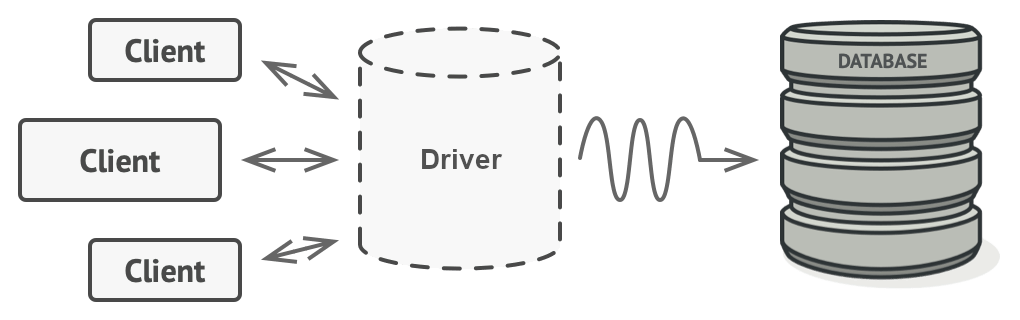
\includegraphics{image.png}
\caption{driver.png}
\end{figure}

\begin{Shaded}
\begin{Highlighting}[]
\CommentTok{// DatabaseDriver.java}

\KeywordTok{package}\ImportTok{ pl}\OperatorTok{.}\ImportTok{edu}\OperatorTok{.}\ImportTok{agh}\OperatorTok{.}\ImportTok{tw}\OperatorTok{.}\ImportTok{knapp}\OperatorTok{.}\ImportTok{lab6}\OperatorTok{;}

\KeywordTok{import} \ImportTok{pl}\OperatorTok{.}\ImportTok{edu}\OperatorTok{.}\ImportTok{agh}\OperatorTok{.}\ImportTok{tw}\OperatorTok{.}\ImportTok{knapp}\OperatorTok{.}\ImportTok{lab6}\OperatorTok{.}\ImportTok{worker}\OperatorTok{.}\ImportTok{Reader}\OperatorTok{;}
\KeywordTok{import} \ImportTok{pl}\OperatorTok{.}\ImportTok{edu}\OperatorTok{.}\ImportTok{agh}\OperatorTok{.}\ImportTok{tw}\OperatorTok{.}\ImportTok{knapp}\OperatorTok{.}\ImportTok{lab6}\OperatorTok{.}\ImportTok{worker}\OperatorTok{.}\ImportTok{Writer}\OperatorTok{;}

\KeywordTok{public} \KeywordTok{abstract} \KeywordTok{class}\NormalTok{ DatabaseDriver}\OperatorTok{\textless{}}\NormalTok{T}\OperatorTok{\textgreater{}} \OperatorTok{\{}
    \KeywordTok{private} \DataTypeTok{final} \DataTypeTok{static} \BuiltInTok{Logger}\NormalTok{ logger }\OperatorTok{=} \BuiltInTok{Logger}\OperatorTok{.}\FunctionTok{getInstance}\OperatorTok{();}

    \KeywordTok{public} \KeywordTok{abstract} \DataTypeTok{boolean} \FunctionTok{read}\OperatorTok{(}\BuiltInTok{Reader}\OperatorTok{\textless{}}\NormalTok{T}\OperatorTok{\textgreater{}}\NormalTok{ reader}\OperatorTok{);}
    \KeywordTok{public} \KeywordTok{abstract} \DataTypeTok{boolean} \FunctionTok{write}\OperatorTok{(}\BuiltInTok{Writer}\OperatorTok{\textless{}}\NormalTok{T}\OperatorTok{\textgreater{}}\NormalTok{ writer}\OperatorTok{);}

    \KeywordTok{protected} \DataTypeTok{void} \FunctionTok{logException}\OperatorTok{(}\BuiltInTok{Exception}\NormalTok{ e}\OperatorTok{)} \OperatorTok{\{}
\NormalTok{        logger}\OperatorTok{.}\FunctionTok{log}\OperatorTok{(}\FunctionTok{getClass}\OperatorTok{().}\FunctionTok{getSimpleName}\OperatorTok{(),}
            \StringTok{"Exception: "} \OperatorTok{+}\NormalTok{ e}\OperatorTok{.}\FunctionTok{getMessage}\OperatorTok{()} \OperatorTok{+} \StringTok{"}\SpecialCharTok{\textbackslash{}n}\StringTok{"} \OperatorTok{+}\NormalTok{ e}\OperatorTok{);}
    \OperatorTok{\}}
\OperatorTok{\}}
\end{Highlighting}
\end{Shaded}

\emph{* -- np. stosuje pewne mechanizmy synchronizacji dostępu do bazy
danych}

    \hypertarget{workert-readert-writert}{%
\subsubsection{\texorpdfstring{\texttt{Worker\textless{}T\textgreater{}},
\texttt{Reader\textless{}T\textgreater{}},
\texttt{Writer\textless{}T\textgreater{}}}{Worker\textless T\textgreater, Reader\textless T\textgreater, Writer\textless T\textgreater{}}}\label{workert-readert-writert}}

Są to interfejsy reprezentujące odpowiednio pracownika, czytelnika i
pisarza.

Implementacja wygląda następująco:

\begin{Shaded}
\begin{Highlighting}[]
\CommentTok{// Worker.java}

\KeywordTok{package}\ImportTok{ pl}\OperatorTok{.}\ImportTok{edu}\OperatorTok{.}\ImportTok{agh}\OperatorTok{.}\ImportTok{tw}\OperatorTok{.}\ImportTok{knapp}\OperatorTok{.}\ImportTok{lab6}\OperatorTok{.}\ImportTok{worker}\OperatorTok{;}

\KeywordTok{import} \ImportTok{pl}\OperatorTok{.}\ImportTok{edu}\OperatorTok{.}\ImportTok{agh}\OperatorTok{.}\ImportTok{tw}\OperatorTok{.}\ImportTok{knapp}\OperatorTok{.}\ImportTok{lab6}\OperatorTok{.}\ImportTok{Database}\OperatorTok{;}

\KeywordTok{public} \KeywordTok{interface}\NormalTok{ Worker}\OperatorTok{\textless{}}\NormalTok{T}\OperatorTok{\textgreater{}} \OperatorTok{\{}
    \DataTypeTok{void} \FunctionTok{work}\OperatorTok{(}\NormalTok{Database}\OperatorTok{\textless{}}\NormalTok{T}\OperatorTok{\textgreater{}}\NormalTok{ db}\OperatorTok{);}
\OperatorTok{\}}
\end{Highlighting}
\end{Shaded}

\begin{Shaded}
\begin{Highlighting}[]
\CommentTok{// Reader.java}

\KeywordTok{package}\ImportTok{ pl}\OperatorTok{.}\ImportTok{edu}\OperatorTok{.}\ImportTok{agh}\OperatorTok{.}\ImportTok{tw}\OperatorTok{.}\ImportTok{knapp}\OperatorTok{.}\ImportTok{lab6}\OperatorTok{.}\ImportTok{worker}\OperatorTok{;}

\KeywordTok{import} \ImportTok{pl}\OperatorTok{.}\ImportTok{edu}\OperatorTok{.}\ImportTok{agh}\OperatorTok{.}\ImportTok{tw}\OperatorTok{.}\ImportTok{knapp}\OperatorTok{.}\ImportTok{lab6}\OperatorTok{.}\ImportTok{Database}\OperatorTok{;}

\KeywordTok{public} \KeywordTok{interface} \BuiltInTok{Reader}\OperatorTok{\textless{}}\NormalTok{T}\OperatorTok{\textgreater{}} \KeywordTok{extends}\NormalTok{ Worker}\OperatorTok{\textless{}}\NormalTok{T}\OperatorTok{\textgreater{}} \OperatorTok{\{}
    \KeywordTok{default} \DataTypeTok{void} \FunctionTok{read}\OperatorTok{(}\NormalTok{Database}\OperatorTok{\textless{}}\NormalTok{T}\OperatorTok{\textgreater{}}\NormalTok{ db}\OperatorTok{)} \OperatorTok{\{}
        \FunctionTok{work}\OperatorTok{(}\NormalTok{db}\OperatorTok{);}
    \OperatorTok{\}}
\OperatorTok{\}}
\end{Highlighting}
\end{Shaded}

\begin{Shaded}
\begin{Highlighting}[]
\CommentTok{// Writer.java}

\KeywordTok{package}\ImportTok{ pl}\OperatorTok{.}\ImportTok{edu}\OperatorTok{.}\ImportTok{agh}\OperatorTok{.}\ImportTok{tw}\OperatorTok{.}\ImportTok{knapp}\OperatorTok{.}\ImportTok{lab6}\OperatorTok{.}\ImportTok{worker}\OperatorTok{;}

\KeywordTok{import} \ImportTok{pl}\OperatorTok{.}\ImportTok{edu}\OperatorTok{.}\ImportTok{agh}\OperatorTok{.}\ImportTok{tw}\OperatorTok{.}\ImportTok{knapp}\OperatorTok{.}\ImportTok{lab6}\OperatorTok{.}\ImportTok{Database}\OperatorTok{;}

\KeywordTok{public} \KeywordTok{interface} \BuiltInTok{Writer}\OperatorTok{\textless{}}\NormalTok{T}\OperatorTok{\textgreater{}} \KeywordTok{extends}\NormalTok{ Worker}\OperatorTok{\textless{}}\NormalTok{T}\OperatorTok{\textgreater{}} \OperatorTok{\{}
    \KeywordTok{default} \DataTypeTok{void} \FunctionTok{write}\OperatorTok{(}\NormalTok{Database}\OperatorTok{\textless{}}\NormalTok{T}\OperatorTok{\textgreater{}}\NormalTok{ db}\OperatorTok{)} \OperatorTok{\{}
        \FunctionTok{work}\OperatorTok{(}\NormalTok{db}\OperatorTok{);}
    \OperatorTok{\}}
\OperatorTok{\}}
\end{Highlighting}
\end{Shaded}

    \hypertarget{workerfactoryt-readerfactoryt-writerfactoryt}{%
\subsubsection{\texorpdfstring{\texttt{WorkerFactory\textless{}T\textgreater{}},
\texttt{ReaderFactory\textless{}T\textgreater{}},
\texttt{WriterFactory\textless{}T\textgreater{}}}{WorkerFactory\textless T\textgreater, ReaderFactory\textless T\textgreater, WriterFactory\textless T\textgreater{}}}\label{workerfactoryt-readerfactoryt-writerfactoryt}}

Są to interfejsy reprezentujące fabryki odpowiednio pracownika,
czytelnika i pisarza. Jak już zostało wspomniane wcześniej, fabruki są
po to, żeby pracownik miał dostęp do numeru iteracji pochodzącego z
odpowiedniego wątku (\texttt{WorkerThread}), co z kolei pozwala podnieść
czytelność logów.

Implementacja wygląda następująco:

\begin{Shaded}
\begin{Highlighting}[]
\CommentTok{// WorkerFactory.java}

\KeywordTok{package}\ImportTok{ pl}\OperatorTok{.}\ImportTok{edu}\OperatorTok{.}\ImportTok{agh}\OperatorTok{.}\ImportTok{tw}\OperatorTok{.}\ImportTok{knapp}\OperatorTok{.}\ImportTok{lab6}\OperatorTok{.}\ImportTok{worker}\OperatorTok{.}\ImportTok{factory}\OperatorTok{;}

\KeywordTok{import} \ImportTok{pl}\OperatorTok{.}\ImportTok{edu}\OperatorTok{.}\ImportTok{agh}\OperatorTok{.}\ImportTok{tw}\OperatorTok{.}\ImportTok{knapp}\OperatorTok{.}\ImportTok{lab6}\OperatorTok{.}\ImportTok{worker}\OperatorTok{.}\ImportTok{Worker}\OperatorTok{;}

\KeywordTok{public} \KeywordTok{interface}\NormalTok{ WorkerFactory}\OperatorTok{\textless{}}\NormalTok{T}\OperatorTok{\textgreater{}} \OperatorTok{\{}
\NormalTok{    Worker}\OperatorTok{\textless{}}\NormalTok{T}\OperatorTok{\textgreater{}} \FunctionTok{get}\OperatorTok{(}\DataTypeTok{int}\NormalTok{ iteration}\OperatorTok{);}
\OperatorTok{\}}
\end{Highlighting}
\end{Shaded}

\begin{Shaded}
\begin{Highlighting}[]
\CommentTok{// ReaderFactory.java}

\KeywordTok{package}\ImportTok{ pl}\OperatorTok{.}\ImportTok{edu}\OperatorTok{.}\ImportTok{agh}\OperatorTok{.}\ImportTok{tw}\OperatorTok{.}\ImportTok{knapp}\OperatorTok{.}\ImportTok{lab6}\OperatorTok{.}\ImportTok{worker}\OperatorTok{.}\ImportTok{factory}\OperatorTok{;}

\KeywordTok{import} \ImportTok{pl}\OperatorTok{.}\ImportTok{edu}\OperatorTok{.}\ImportTok{agh}\OperatorTok{.}\ImportTok{tw}\OperatorTok{.}\ImportTok{knapp}\OperatorTok{.}\ImportTok{lab6}\OperatorTok{.}\ImportTok{worker}\OperatorTok{.}\ImportTok{Reader}\OperatorTok{;}

\KeywordTok{public} \KeywordTok{interface}\NormalTok{ ReaderFactory}\OperatorTok{\textless{}}\NormalTok{T}\OperatorTok{\textgreater{}} \KeywordTok{extends}\NormalTok{ WorkerFactory}\OperatorTok{\textless{}}\NormalTok{T}\OperatorTok{\textgreater{}} \OperatorTok{\{}
    \AttributeTok{@Override}
    \BuiltInTok{Reader}\OperatorTok{\textless{}}\NormalTok{T}\OperatorTok{\textgreater{}} \FunctionTok{get}\OperatorTok{(}\DataTypeTok{int}\NormalTok{ iteration}\OperatorTok{);}
\OperatorTok{\}}
\end{Highlighting}
\end{Shaded}

\begin{Shaded}
\begin{Highlighting}[]
\CommentTok{// WriterFactory.java}

\KeywordTok{package}\ImportTok{ pl}\OperatorTok{.}\ImportTok{edu}\OperatorTok{.}\ImportTok{agh}\OperatorTok{.}\ImportTok{tw}\OperatorTok{.}\ImportTok{knapp}\OperatorTok{.}\ImportTok{lab6}\OperatorTok{.}\ImportTok{worker}\OperatorTok{.}\ImportTok{factory}\OperatorTok{;}

\KeywordTok{import} \ImportTok{pl}\OperatorTok{.}\ImportTok{edu}\OperatorTok{.}\ImportTok{agh}\OperatorTok{.}\ImportTok{tw}\OperatorTok{.}\ImportTok{knapp}\OperatorTok{.}\ImportTok{lab6}\OperatorTok{.}\ImportTok{worker}\OperatorTok{.}\ImportTok{Writer}\OperatorTok{;}

\KeywordTok{public} \KeywordTok{interface}\NormalTok{ WriterFactory}\OperatorTok{\textless{}}\NormalTok{T}\OperatorTok{\textgreater{}} \KeywordTok{extends}\NormalTok{ WorkerFactory}\OperatorTok{\textless{}}\NormalTok{T}\OperatorTok{\textgreater{}} \OperatorTok{\{}
    \AttributeTok{@Override}
    \BuiltInTok{Writer}\OperatorTok{\textless{}}\NormalTok{T}\OperatorTok{\textgreater{}} \FunctionTok{get}\OperatorTok{(}\DataTypeTok{int}\NormalTok{ iteration}\OperatorTok{);}
\OperatorTok{\}}
\end{Highlighting}
\end{Shaded}

    \hypertarget{workerthreadt-readerthreadt-writerthreadt}{%
\subsubsection{\texorpdfstring{\texttt{WorkerThread\textless{}T\textgreater{}},
\texttt{ReaderThread\textless{}T\textgreater{}},
\texttt{WriterThread\textless{}T\textgreater{}}}{WorkerThread\textless T\textgreater, ReaderThread\textless T\textgreater, WriterThread\textless T\textgreater{}}}\label{workerthreadt-readerthreadt-writerthreadt}}

\texttt{WorkerThread} jest to abstrakcyjna klasa nadrzędna,
reprezentująca wątek pracownika. Wykonuje zadaną liczbę iteracji, po
każdej iteracji wątek zostaje uśpiony na pewien czas, losowany z
zadanego przedziału. Posiada metodę abstrakcyjną
\texttt{void\ onIter(int\ i)}, która jest wywoływana co każdą iterację,
\texttt{i} - numer tej iteracji.

\texttt{ReaderThread} i \texttt{WriterThread} dziedziczą po klasie
\texttt{WorkerThread} i implementują metodę \texttt{onIter}.

Implementacje wszystkich trzech klas wyglądają następująco:

\begin{Shaded}
\begin{Highlighting}[]
\CommentTok{// WorkerThread.java}

\KeywordTok{package}\ImportTok{ pl}\OperatorTok{.}\ImportTok{edu}\OperatorTok{.}\ImportTok{agh}\OperatorTok{.}\ImportTok{tw}\OperatorTok{.}\ImportTok{knapp}\OperatorTok{.}\ImportTok{lab6}\OperatorTok{.}\ImportTok{worker}\OperatorTok{.}\ImportTok{thread}\OperatorTok{;}

\KeywordTok{import} \ImportTok{pl}\OperatorTok{.}\ImportTok{edu}\OperatorTok{.}\ImportTok{agh}\OperatorTok{.}\ImportTok{tw}\OperatorTok{.}\ImportTok{knapp}\OperatorTok{.}\ImportTok{lab6}\OperatorTok{.}\ImportTok{DatabaseDriver}\OperatorTok{;}
\KeywordTok{import} \ImportTok{pl}\OperatorTok{.}\ImportTok{edu}\OperatorTok{.}\ImportTok{agh}\OperatorTok{.}\ImportTok{tw}\OperatorTok{.}\ImportTok{knapp}\OperatorTok{.}\ImportTok{lab6}\OperatorTok{.}\ImportTok{RandomSleeper}\OperatorTok{;}
\KeywordTok{import} \ImportTok{pl}\OperatorTok{.}\ImportTok{edu}\OperatorTok{.}\ImportTok{agh}\OperatorTok{.}\ImportTok{tw}\OperatorTok{.}\ImportTok{knapp}\OperatorTok{.}\ImportTok{lab6}\OperatorTok{.}\ImportTok{worker}\OperatorTok{.}\ImportTok{factory}\OperatorTok{.}\ImportTok{WorkerFactory}\OperatorTok{;}

\KeywordTok{public} \KeywordTok{abstract} \KeywordTok{class}\NormalTok{ WorkerThread}\OperatorTok{\textless{}}\NormalTok{T}\OperatorTok{\textgreater{}} \KeywordTok{extends} \BuiltInTok{Thread} \OperatorTok{\{}
    \KeywordTok{protected} \DataTypeTok{final}\NormalTok{ WorkerFactory}\OperatorTok{\textless{}}\NormalTok{T}\OperatorTok{\textgreater{}}\NormalTok{ factory}\OperatorTok{;}
    \KeywordTok{protected} \DataTypeTok{final}\NormalTok{ DatabaseDriver}\OperatorTok{\textless{}}\NormalTok{T}\OperatorTok{\textgreater{}}\NormalTok{ driver}\OperatorTok{;}
    \KeywordTok{private} \DataTypeTok{final}\NormalTok{ RandomSleeper sleeper}\OperatorTok{;}
    \KeywordTok{private} \DataTypeTok{final} \DataTypeTok{int}\NormalTok{ iterCount}\OperatorTok{;}

    \KeywordTok{public} \FunctionTok{WorkerThread}\OperatorTok{(}\NormalTok{WorkerFactory}\OperatorTok{\textless{}}\NormalTok{T}\OperatorTok{\textgreater{}}\NormalTok{ factory}\OperatorTok{,}\NormalTok{ DatabaseDriver}\OperatorTok{\textless{}}\NormalTok{T}\OperatorTok{\textgreater{}}\NormalTok{ driver}\OperatorTok{,}
                        \DataTypeTok{int}\NormalTok{ delayMinMs}\OperatorTok{,} \DataTypeTok{int}\NormalTok{ delayMaxMs}\OperatorTok{,} \DataTypeTok{int}\NormalTok{ iterCount}\OperatorTok{)}
    \OperatorTok{\{}
        \KeywordTok{this}\OperatorTok{.}\FunctionTok{factory} \OperatorTok{=}\NormalTok{ factory}\OperatorTok{;}
        \KeywordTok{this}\OperatorTok{.}\FunctionTok{driver} \OperatorTok{=}\NormalTok{ driver}\OperatorTok{;}
        \KeywordTok{this}\OperatorTok{.}\FunctionTok{sleeper} \OperatorTok{=} \KeywordTok{new} \FunctionTok{RandomSleeper}\OperatorTok{(}\NormalTok{delayMinMs}\OperatorTok{,}\NormalTok{ delayMaxMs}\OperatorTok{);}
        \KeywordTok{this}\OperatorTok{.}\FunctionTok{iterCount} \OperatorTok{=}\NormalTok{ iterCount}\OperatorTok{;}
    \OperatorTok{\}}

    \AttributeTok{@Override}
    \KeywordTok{public} \DataTypeTok{void} \FunctionTok{run}\OperatorTok{()} \OperatorTok{\{}
        \ControlFlowTok{for} \OperatorTok{(}\DataTypeTok{int}\NormalTok{ i }\OperatorTok{=} \DecValTok{0}\OperatorTok{;}\NormalTok{ i }\OperatorTok{\textless{}}\NormalTok{ iterCount}\OperatorTok{;} \OperatorTok{++}\NormalTok{i}\OperatorTok{)} \OperatorTok{\{}
            \FunctionTok{onIter}\OperatorTok{(}\NormalTok{i}\OperatorTok{);}

            \ControlFlowTok{try} \OperatorTok{\{}
\NormalTok{                sleeper}\OperatorTok{.}\FunctionTok{sleep}\OperatorTok{();}
            \OperatorTok{\}} \ControlFlowTok{catch} \OperatorTok{(}\BuiltInTok{InterruptedException}\NormalTok{ e}\OperatorTok{)} \OperatorTok{\{}
                \ControlFlowTok{throw} \KeywordTok{new} \BuiltInTok{RuntimeException}\OperatorTok{(}\NormalTok{e}\OperatorTok{);}
            \OperatorTok{\}}
        \OperatorTok{\}}
    \OperatorTok{\}}

    \KeywordTok{protected} \KeywordTok{abstract} \DataTypeTok{void} \FunctionTok{onIter}\OperatorTok{(}\DataTypeTok{int}\NormalTok{ i}\OperatorTok{);}
\OperatorTok{\}}
\end{Highlighting}
\end{Shaded}

\begin{Shaded}
\begin{Highlighting}[]
\CommentTok{// ReaderThread.java}

\KeywordTok{package}\ImportTok{ pl}\OperatorTok{.}\ImportTok{edu}\OperatorTok{.}\ImportTok{agh}\OperatorTok{.}\ImportTok{tw}\OperatorTok{.}\ImportTok{knapp}\OperatorTok{.}\ImportTok{lab6}\OperatorTok{.}\ImportTok{worker}\OperatorTok{.}\ImportTok{thread}\OperatorTok{;}

\KeywordTok{import} \ImportTok{pl}\OperatorTok{.}\ImportTok{edu}\OperatorTok{.}\ImportTok{agh}\OperatorTok{.}\ImportTok{tw}\OperatorTok{.}\ImportTok{knapp}\OperatorTok{.}\ImportTok{lab6}\OperatorTok{.}\ImportTok{DatabaseDriver}\OperatorTok{;}
\KeywordTok{import} \ImportTok{pl}\OperatorTok{.}\ImportTok{edu}\OperatorTok{.}\ImportTok{agh}\OperatorTok{.}\ImportTok{tw}\OperatorTok{.}\ImportTok{knapp}\OperatorTok{.}\ImportTok{lab6}\OperatorTok{.}\ImportTok{worker}\OperatorTok{.}\ImportTok{Reader}\OperatorTok{;}
\KeywordTok{import} \ImportTok{pl}\OperatorTok{.}\ImportTok{edu}\OperatorTok{.}\ImportTok{agh}\OperatorTok{.}\ImportTok{tw}\OperatorTok{.}\ImportTok{knapp}\OperatorTok{.}\ImportTok{lab6}\OperatorTok{.}\ImportTok{worker}\OperatorTok{.}\ImportTok{factory}\OperatorTok{.}\ImportTok{ReaderFactory}\OperatorTok{;}

\KeywordTok{public} \KeywordTok{class}\NormalTok{ ReaderThread}\OperatorTok{\textless{}}\NormalTok{T}\OperatorTok{\textgreater{}} \KeywordTok{extends}\NormalTok{ WorkerThread}\OperatorTok{\textless{}}\NormalTok{T}\OperatorTok{\textgreater{}} \OperatorTok{\{}
    \KeywordTok{public} \FunctionTok{ReaderThread}\OperatorTok{(}\NormalTok{ReaderFactory}\OperatorTok{\textless{}}\NormalTok{T}\OperatorTok{\textgreater{}}\NormalTok{ factory}\OperatorTok{,}\NormalTok{ DatabaseDriver}\OperatorTok{\textless{}}\NormalTok{T}\OperatorTok{\textgreater{}}\NormalTok{ driver}\OperatorTok{,}
                        \DataTypeTok{int}\NormalTok{ delayMinMs}\OperatorTok{,} \DataTypeTok{int}\NormalTok{ delayMaxMs}\OperatorTok{,} \DataTypeTok{int}\NormalTok{ iterCount}\OperatorTok{)}
    \OperatorTok{\{}
        \KeywordTok{super}\OperatorTok{(}\NormalTok{factory}\OperatorTok{,}\NormalTok{ driver}\OperatorTok{,}\NormalTok{ delayMinMs}\OperatorTok{,}\NormalTok{ delayMaxMs}\OperatorTok{,}\NormalTok{ iterCount}\OperatorTok{);}
    \OperatorTok{\}}

    \AttributeTok{@Override}
    \KeywordTok{protected} \DataTypeTok{void} \FunctionTok{onIter}\OperatorTok{(}\DataTypeTok{int}\NormalTok{ i}\OperatorTok{)} \OperatorTok{\{}
\NormalTok{        driver}\OperatorTok{.}\FunctionTok{read}\OperatorTok{((}\BuiltInTok{Reader}\OperatorTok{\textless{}}\NormalTok{T}\OperatorTok{\textgreater{})}\NormalTok{ factory}\OperatorTok{.}\FunctionTok{get}\OperatorTok{(}\NormalTok{i}\OperatorTok{));}
    \OperatorTok{\}}
\OperatorTok{\}}
\end{Highlighting}
\end{Shaded}

\begin{Shaded}
\begin{Highlighting}[]
\CommentTok{// WriterThread.java}

\KeywordTok{package}\ImportTok{ pl}\OperatorTok{.}\ImportTok{edu}\OperatorTok{.}\ImportTok{agh}\OperatorTok{.}\ImportTok{tw}\OperatorTok{.}\ImportTok{knapp}\OperatorTok{.}\ImportTok{lab6}\OperatorTok{.}\ImportTok{worker}\OperatorTok{.}\ImportTok{thread}\OperatorTok{;}

\KeywordTok{import} \ImportTok{pl}\OperatorTok{.}\ImportTok{edu}\OperatorTok{.}\ImportTok{agh}\OperatorTok{.}\ImportTok{tw}\OperatorTok{.}\ImportTok{knapp}\OperatorTok{.}\ImportTok{lab6}\OperatorTok{.}\ImportTok{DatabaseDriver}\OperatorTok{;}
\KeywordTok{import} \ImportTok{pl}\OperatorTok{.}\ImportTok{edu}\OperatorTok{.}\ImportTok{agh}\OperatorTok{.}\ImportTok{tw}\OperatorTok{.}\ImportTok{knapp}\OperatorTok{.}\ImportTok{lab6}\OperatorTok{.}\ImportTok{worker}\OperatorTok{.}\ImportTok{Writer}\OperatorTok{;}
\KeywordTok{import} \ImportTok{pl}\OperatorTok{.}\ImportTok{edu}\OperatorTok{.}\ImportTok{agh}\OperatorTok{.}\ImportTok{tw}\OperatorTok{.}\ImportTok{knapp}\OperatorTok{.}\ImportTok{lab6}\OperatorTok{.}\ImportTok{worker}\OperatorTok{.}\ImportTok{factory}\OperatorTok{.}\ImportTok{WriterFactory}\OperatorTok{;}

\KeywordTok{public} \KeywordTok{class}\NormalTok{ WriterThread}\OperatorTok{\textless{}}\NormalTok{T}\OperatorTok{\textgreater{}} \KeywordTok{extends}\NormalTok{ WorkerThread}\OperatorTok{\textless{}}\NormalTok{T}\OperatorTok{\textgreater{}} \OperatorTok{\{}
    \KeywordTok{public} \FunctionTok{WriterThread}\OperatorTok{(}\NormalTok{WriterFactory}\OperatorTok{\textless{}}\NormalTok{T}\OperatorTok{\textgreater{}}\NormalTok{ factory}\OperatorTok{,}\NormalTok{ DatabaseDriver}\OperatorTok{\textless{}}\NormalTok{T}\OperatorTok{\textgreater{}}\NormalTok{ driver}\OperatorTok{,}
                        \DataTypeTok{int}\NormalTok{ delayMinMs}\OperatorTok{,} \DataTypeTok{int}\NormalTok{ delayMaxMs}\OperatorTok{,} \DataTypeTok{int}\NormalTok{ iterCount}\OperatorTok{)}
    \OperatorTok{\{}
        \KeywordTok{super}\OperatorTok{(}\NormalTok{factory}\OperatorTok{,}\NormalTok{ driver}\OperatorTok{,}\NormalTok{ delayMinMs}\OperatorTok{,}\NormalTok{ delayMaxMs}\OperatorTok{,}\NormalTok{ iterCount}\OperatorTok{);}
    \OperatorTok{\}}

    \AttributeTok{@Override}
    \KeywordTok{protected} \DataTypeTok{void} \FunctionTok{onIter}\OperatorTok{(}\DataTypeTok{int}\NormalTok{ i}\OperatorTok{)} \OperatorTok{\{}
\NormalTok{        driver}\OperatorTok{.}\FunctionTok{write}\OperatorTok{((}\BuiltInTok{Writer}\OperatorTok{\textless{}}\NormalTok{T}\OperatorTok{\textgreater{})}\NormalTok{ factory}\OperatorTok{.}\FunctionTok{get}\OperatorTok{(}\NormalTok{i}\OperatorTok{));}
    \OperatorTok{\}}
\OperatorTok{\}}
\end{Highlighting}
\end{Shaded}

    \hypertarget{logger}{%
\subsubsection{\texorpdfstring{\texttt{Logger}}{Logger}}\label{logger}}

Jest to klasa służąca do tworzenia logów. Podczas implementacji, w
celach ułatwienia zarządzaniem logami, użyto wzorca \emph{Singleton}.

\begin{Shaded}
\begin{Highlighting}[]
\CommentTok{// Logger.java}

\KeywordTok{package}\ImportTok{ pl}\OperatorTok{.}\ImportTok{edu}\OperatorTok{.}\ImportTok{agh}\OperatorTok{.}\ImportTok{tw}\OperatorTok{.}\ImportTok{knapp}\OperatorTok{.}\ImportTok{lab5}\OperatorTok{;}

\KeywordTok{import} \ImportTok{java}\OperatorTok{.}\ImportTok{util}\OperatorTok{.}\ImportTok{function}\OperatorTok{.}\ImportTok{Consumer}\OperatorTok{;}

\KeywordTok{public} \KeywordTok{class} \BuiltInTok{Logger} \OperatorTok{\{}
    \KeywordTok{private} \DataTypeTok{static} \DataTypeTok{final} \BuiltInTok{Logger}\NormalTok{ logger }\OperatorTok{=} \KeywordTok{new} \BuiltInTok{Logger}\OperatorTok{();}

    \KeywordTok{private}\NormalTok{ Consumer}\OperatorTok{\textless{}}\BuiltInTok{String}\OperatorTok{\textgreater{}}\NormalTok{ consumer }\OperatorTok{=} \FunctionTok{defaultConsumer}\OperatorTok{();}

    \KeywordTok{private} \DataTypeTok{static}\NormalTok{ Consumer}\OperatorTok{\textless{}}\BuiltInTok{String}\OperatorTok{\textgreater{}} \FunctionTok{defaultConsumer}\OperatorTok{()} \OperatorTok{\{}
        \ControlFlowTok{return} \BuiltInTok{System}\OperatorTok{.}\FunctionTok{out}\OperatorTok{::}\NormalTok{println}\OperatorTok{;}
    \OperatorTok{\}}

    \KeywordTok{private} \BuiltInTok{Logger}\OperatorTok{()} \OperatorTok{\{}
        \CommentTok{// empty}
    \OperatorTok{\}}

    \KeywordTok{public} \DataTypeTok{void} \FunctionTok{log}\OperatorTok{(}\BuiltInTok{String}\NormalTok{ tag}\OperatorTok{,} \BuiltInTok{Object}\NormalTok{ o}\OperatorTok{)} \OperatorTok{\{}
\NormalTok{        consumer}\OperatorTok{.}\FunctionTok{accept}\OperatorTok{(}\BuiltInTok{String}\OperatorTok{.}\FunctionTok{format}\OperatorTok{(}\StringTok{"[}\SpecialCharTok{\%s}\StringTok{] }\SpecialCharTok{\%s}\StringTok{"}\OperatorTok{,}\NormalTok{ tag}\OperatorTok{,}\NormalTok{ o}\OperatorTok{));}
    \OperatorTok{\}}

    \KeywordTok{public} \DataTypeTok{void} \FunctionTok{log}\OperatorTok{(}\BuiltInTok{Object}\NormalTok{ o}\OperatorTok{)} \OperatorTok{\{}
\NormalTok{        consumer}\OperatorTok{.}\FunctionTok{accept}\OperatorTok{(}\BuiltInTok{String}\OperatorTok{.}\FunctionTok{valueOf}\OperatorTok{(}\NormalTok{o}\OperatorTok{));}
    \OperatorTok{\}}

    \KeywordTok{public} \DataTypeTok{void} \FunctionTok{setConsumer}\OperatorTok{(}\NormalTok{Consumer}\OperatorTok{\textless{}}\BuiltInTok{String}\OperatorTok{\textgreater{}}\NormalTok{ consumer}\OperatorTok{)} \OperatorTok{\{}
        \KeywordTok{this}\OperatorTok{.}\FunctionTok{consumer} \OperatorTok{=}\NormalTok{ consumer}\OperatorTok{;}
    \OperatorTok{\}}

    \KeywordTok{public} \DataTypeTok{void} \FunctionTok{mute}\OperatorTok{()} \OperatorTok{\{}
        \FunctionTok{setConsumer}\OperatorTok{(}\NormalTok{s }\OperatorTok{{-}\textgreater{}} \OperatorTok{\{\});}
    \OperatorTok{\}}

    \KeywordTok{public} \DataTypeTok{void} \FunctionTok{unmute}\OperatorTok{()} \OperatorTok{\{}
        \FunctionTok{setConsumer}\OperatorTok{(}\FunctionTok{defaultConsumer}\OperatorTok{());}
    \OperatorTok{\}}

    \KeywordTok{public} \DataTypeTok{static} \BuiltInTok{Logger} \FunctionTok{getInstance}\OperatorTok{()} \OperatorTok{\{}
        \ControlFlowTok{return}\NormalTok{ logger}\OperatorTok{;}
    \OperatorTok{\}}
\OperatorTok{\}}
\end{Highlighting}
\end{Shaded}

Jak i w przypadku poprzedniego laboratorium,

\begin{itemize}
\tightlist
\item
  \texttt{log(String\ tag,\ Object\ o)} wypisuje log wraz z tagiem (np.
  \emph{Philosopher \#5}. Chodzi tu o rozpoznawanie źródła pochodzenia
  informacji). Obiekt \texttt{o} może mieć wartość \texttt{null}.
\item
  \texttt{log(Object\ o)} wypisuje tekstową reprezentację obiektu
  \texttt{o}. Obiekt \texttt{o} może mieć wartość \texttt{null}.
\item
  \texttt{setConsumer(Consumer\textless{}String\textgreater{}\ consumer)}
  umożliwia ustawienie kastomowego konsumenta logów
\item
  \texttt{mute()} wycisza Logger
\item
  \texttt{unmute()} przeciwieństwo metody \texttt{mute}: jako konsument
  zostanie użyta domyślna implementacja wypisująca na standardowym
  wyjściu
\item
  \texttt{getInstance()} zwraca instancję klasy \texttt{Logger}
\end{itemize}

    \hypertarget{randomsleeper}{%
\subsubsection{\texorpdfstring{\texttt{RandomSleeper}}{RandomSleeper}}\label{randomsleeper}}

Klasa służąca do uśpienia wątku na pewien czas, losowany z przedziału
\texttt{{[}delayMinMs,\ delayMaxMs)}.

\begin{Shaded}
\begin{Highlighting}[]
\CommentTok{// RandomSleeper.java}

\KeywordTok{package}\ImportTok{ pl}\OperatorTok{.}\ImportTok{edu}\OperatorTok{.}\ImportTok{agh}\OperatorTok{.}\ImportTok{tw}\OperatorTok{.}\ImportTok{knapp}\OperatorTok{.}\ImportTok{lab5}\OperatorTok{;}

\KeywordTok{import} \ImportTok{java}\OperatorTok{.}\ImportTok{util}\OperatorTok{.}\ImportTok{Random}\OperatorTok{;}

\KeywordTok{public} \KeywordTok{class}\NormalTok{ RandomSleeper }\OperatorTok{\{}
    \KeywordTok{private} \DataTypeTok{final} \BuiltInTok{Random}\NormalTok{ delayRandom }\OperatorTok{=} \KeywordTok{new} \BuiltInTok{Random}\OperatorTok{();}
    \KeywordTok{private} \DataTypeTok{final} \DataTypeTok{long}\NormalTok{ delayMinMs}\OperatorTok{;}
    \KeywordTok{private} \DataTypeTok{final} \DataTypeTok{long}\NormalTok{ delayMaxMs}\OperatorTok{;}

    \KeywordTok{public} \FunctionTok{RandomSleeper}\OperatorTok{(}\DataTypeTok{long}\NormalTok{ delayMinMs}\OperatorTok{,} \DataTypeTok{long}\NormalTok{ delayMaxMs}\OperatorTok{)} \OperatorTok{\{}
        \KeywordTok{this}\OperatorTok{.}\FunctionTok{delayMinMs} \OperatorTok{=}\NormalTok{ delayMinMs}\OperatorTok{;}
        \KeywordTok{this}\OperatorTok{.}\FunctionTok{delayMaxMs} \OperatorTok{=}\NormalTok{ delayMaxMs}\OperatorTok{;}
    \OperatorTok{\}}

    \KeywordTok{public} \DataTypeTok{void} \FunctionTok{sleep}\OperatorTok{()} \KeywordTok{throws} \BuiltInTok{InterruptedException} \OperatorTok{\{}
        \ControlFlowTok{if} \OperatorTok{(}\NormalTok{delayMinMs }\OperatorTok{==} \DecValTok{0} \OperatorTok{\&\&}\NormalTok{ delayMaxMs }\OperatorTok{==} \DecValTok{0}\OperatorTok{)}
            \ControlFlowTok{return}\OperatorTok{;}
        \DataTypeTok{var}\NormalTok{ delay }\OperatorTok{=}\NormalTok{ delayRandom}\OperatorTok{.}\FunctionTok{nextLong}\OperatorTok{(}\NormalTok{delayMinMs}\OperatorTok{,}\NormalTok{ delayMaxMs}\OperatorTok{);}
        \BuiltInTok{Thread}\OperatorTok{.}\FunctionTok{sleep}\OperatorTok{(}\NormalTok{delay}\OperatorTok{);}
    \OperatorTok{\}}
\OperatorTok{\}}
\end{Highlighting}
\end{Shaded}

    \hypertarget{rozwiux105zania-z-jednym-zamkiem}{%
\subsection{Rozwiązania z jednym
zamkiem}\label{rozwiux105zania-z-jednym-zamkiem}}

W tym rozdziale zostaną zaprezentowane i opisane 2 rozwiązania z jednym
zamkiem: zaimplementowane w oparciu o semafory i zmienne warunkowe.

    \hypertarget{simpledatabaset}{%
\subsubsection{\texorpdfstring{\texttt{SimpleDatabase\textless{}T\textgreater{}}}{SimpleDatabase\textless T\textgreater{}}}\label{simpledatabaset}}

Jest to klasa implementująca interfejs \texttt{Database}. W tym
przypadku jest to zwykły wrapper dla listy typu
\texttt{LinkedList\textless{}T\textgreater{}}.

Implementacja wygląda w następujący sposób:

\begin{Shaded}
\begin{Highlighting}[]
\CommentTok{// SimpleDatabase.java}

\KeywordTok{package}\ImportTok{ pl}\OperatorTok{.}\ImportTok{edu}\OperatorTok{.}\ImportTok{agh}\OperatorTok{.}\ImportTok{tw}\OperatorTok{.}\ImportTok{knapp}\OperatorTok{.}\ImportTok{lab6}\OperatorTok{.}\ImportTok{blocking}\OperatorTok{;}

\KeywordTok{import} \ImportTok{pl}\OperatorTok{.}\ImportTok{edu}\OperatorTok{.}\ImportTok{agh}\OperatorTok{.}\ImportTok{tw}\OperatorTok{.}\ImportTok{knapp}\OperatorTok{.}\ImportTok{lab6}\OperatorTok{.}\ImportTok{Database}\OperatorTok{;}

\KeywordTok{import} \ImportTok{java}\OperatorTok{.}\ImportTok{util}\OperatorTok{.}\ImportTok{LinkedList}\OperatorTok{;}
\KeywordTok{import} \ImportTok{java}\OperatorTok{.}\ImportTok{util}\OperatorTok{.}\ImportTok{List}\OperatorTok{;}
\KeywordTok{import} \ImportTok{java}\OperatorTok{.}\ImportTok{util}\OperatorTok{.}\ImportTok{function}\OperatorTok{.}\ImportTok{Consumer}\OperatorTok{;}

\KeywordTok{public} \KeywordTok{class}\NormalTok{ SimpleDatabase}\OperatorTok{\textless{}}\NormalTok{T}\OperatorTok{\textgreater{}} \KeywordTok{implements}\NormalTok{ Database}\OperatorTok{\textless{}}\NormalTok{T}\OperatorTok{\textgreater{}} \OperatorTok{\{}
    \KeywordTok{private} \DataTypeTok{final} \BuiltInTok{List}\OperatorTok{\textless{}}\NormalTok{T}\OperatorTok{\textgreater{}}\NormalTok{ data }\OperatorTok{=} \KeywordTok{new} \BuiltInTok{LinkedList}\OperatorTok{\textless{}\textgreater{}();}

    \AttributeTok{@Override}
    \KeywordTok{public} \OperatorTok{\textless{}}\NormalTok{E }\KeywordTok{extends}\NormalTok{ T}\OperatorTok{\textgreater{}} \DataTypeTok{boolean} \FunctionTok{contains}\OperatorTok{(}\NormalTok{E element}\OperatorTok{)} \OperatorTok{\{}
        \ControlFlowTok{return}\NormalTok{ data}\OperatorTok{.}\FunctionTok{contains}\OperatorTok{(}\NormalTok{element}\OperatorTok{);}
    \OperatorTok{\}}

    \AttributeTok{@Override}
    \KeywordTok{public} \OperatorTok{\textless{}}\NormalTok{E }\KeywordTok{extends}\NormalTok{ T}\OperatorTok{\textgreater{}} \DataTypeTok{boolean} \FunctionTok{remove}\OperatorTok{(}\NormalTok{E element}\OperatorTok{)} \OperatorTok{\{}
        \ControlFlowTok{return}\NormalTok{ data}\OperatorTok{.}\FunctionTok{remove}\OperatorTok{(}\NormalTok{element}\OperatorTok{);}
    \OperatorTok{\}}

    \AttributeTok{@Override}
    \KeywordTok{public} \OperatorTok{\textless{}}\NormalTok{E }\KeywordTok{extends}\NormalTok{ T}\OperatorTok{\textgreater{}} \DataTypeTok{boolean} \FunctionTok{add}\OperatorTok{(}\NormalTok{E element}\OperatorTok{)} \OperatorTok{\{}
        \ControlFlowTok{return}\NormalTok{ data}\OperatorTok{.}\FunctionTok{add}\OperatorTok{(}\NormalTok{element}\OperatorTok{);}
    \OperatorTok{\}}

    \AttributeTok{@Override}
    \KeywordTok{public} \DataTypeTok{void} \FunctionTok{forEach}\OperatorTok{(}\NormalTok{Consumer}\OperatorTok{\textless{}?} \KeywordTok{super}\NormalTok{ T}\OperatorTok{\textgreater{}}\NormalTok{ consumer}\OperatorTok{)} \OperatorTok{\{}
\NormalTok{        data}\OperatorTok{.}\FunctionTok{forEach}\OperatorTok{(}\NormalTok{consumer}\OperatorTok{);}
    \OperatorTok{\}}
\OperatorTok{\}}
\end{Highlighting}
\end{Shaded}

    \hypertarget{blockingdatabasedrivert}{%
\subsubsection{\texorpdfstring{\texttt{BlockingDatabaseDriver\textless{}T\textgreater{}}}{BlockingDatabaseDriver\textless T\textgreater{}}}\label{blockingdatabasedrivert}}

Jest to driver reprezentujący rozwiązanie z wykorzystaniem semaforów.
Dziedziczy po \texttt{DatabaseDriver}.

Zostały użyte 3 semafory o wartości początkowej \texttt{1}:

\begin{enumerate}
\def\labelenumi{\arabic{enumi}.}
\tightlist
\item
  \texttt{resource}: służy do zarządzania dostępem do zasobu (bazy
  danych)
\item
  \texttt{readCountLock}: służy do zsynchronizowanego dostępu do
  licznika aktywnych czytelników
\item
  \texttt{serviceQueue}: służy do kolejkowania pracowników (jest do
  możliwe dzieki temu, że semafory w Javie mogą się zachowywać jak
  kolejki FIFO*). Właśnie dzieki temu semaforowi nie zostanie zagłodzona
  żadna kategoria pracowników.
\end{enumerate}

\emph{* -- dokładniej mówiąc, ten semafor został stworzony w sposób,
gwarantujący kolejność FIFO.}

\textbf{Opis algorytmu:}

\begin{itemize}
\tightlist
\item
  Każdy pracownik najpierw ``wchodzi do kolejki'' blokując
  \texttt{serviceQueue}
\item
  Jeżeli to jest pisarz, to:

  \begin{itemize}
  \tightlist
  \item
    Blokuje semafor \texttt{resource}
  \item
    Odblokowuje \texttt{serviceQueue}
  \item
    Pisze do bazy danych
  \item
    Odblokowuje \texttt{resource}
  \end{itemize}
\item
  Jeżeli to jest czytelnik, to sprawa trochę bardziej się komplikuje:

  \begin{itemize}
  \tightlist
  \item
    Blokuje \texttt{serviceQueue}
  \item
    Blokuje \texttt{readCountLock}
  \item
    Zwiększa licznik \texttt{readCount} o \texttt{1}
  \item
    Jeżeli \texttt{readCount\ ==\ 1}, to blokuje \texttt{resource}. To
    znaczy, że ten czytelnik ``wchodzi do pustej sali''
  \item
    Odblokowuje \texttt{serviceQueue}
  \item
    Odblokowuje \texttt{readCountLock}
  \item
    Czyta z bazy danych
  \item
    Blokuje \texttt{readCountLock}
  \item
    Zmniejsza licznik \texttt{readCount} o \texttt{1}
  \item
    Jeżeli \texttt{readCount\ ==\ 0}, to odblokowuje \texttt{resource}.
    To znaczy, że ``wychodzi z sali jako ostatni''
  \item
    Odblokowuje \texttt{readCountLock}
  \end{itemize}
\end{itemize}

Jak już zostało wspomniane wcześniej, \texttt{serviceQueue} zachowuje
się jak kolejka \texttt{FIFO}. Zgodnie z dokumentacją, został użyty
następujący konstruktor z wartością \texttt{fair} ustawioną na
\texttt{true}:

\begin{quote}
\begin{Shaded}
\begin{Highlighting}[]
\KeywordTok{public} \BuiltInTok{Semaphore}\OperatorTok{(}\DataTypeTok{int}\NormalTok{ permits}\OperatorTok{,} \DataTypeTok{boolean}\NormalTok{ fair}\OperatorTok{)}
\end{Highlighting}
\end{Shaded}

Creates a Semaphore with the given number of permits and the given
fairness setting.

Parameters:

\begin{itemize}
\tightlist
\item
  \textbf{\texttt{permits}} - the initial number of permits available.
  This value may be negative, in which case releases must occur before
  any acquires will be granted.
\item
  \textbf{\texttt{fair}} - \texttt{true} if this semaphore will
  guarantee first-in first-out granting of permits under contention,
  else \texttt{false}
\end{itemize}
\end{quote}

Implementacja wygląda następująco:

\begin{Shaded}
\begin{Highlighting}[]
\CommentTok{// BlockingDatabaseDriver.java}

\KeywordTok{package}\ImportTok{ pl}\OperatorTok{.}\ImportTok{edu}\OperatorTok{.}\ImportTok{agh}\OperatorTok{.}\ImportTok{tw}\OperatorTok{.}\ImportTok{knapp}\OperatorTok{.}\ImportTok{lab6}\OperatorTok{.}\ImportTok{blocking}\OperatorTok{;}

\KeywordTok{import} \ImportTok{pl}\OperatorTok{.}\ImportTok{edu}\OperatorTok{.}\ImportTok{agh}\OperatorTok{.}\ImportTok{tw}\OperatorTok{.}\ImportTok{knapp}\OperatorTok{.}\ImportTok{lab6}\OperatorTok{.*;}
\KeywordTok{import} \ImportTok{pl}\OperatorTok{.}\ImportTok{edu}\OperatorTok{.}\ImportTok{agh}\OperatorTok{.}\ImportTok{tw}\OperatorTok{.}\ImportTok{knapp}\OperatorTok{.}\ImportTok{lab6}\OperatorTok{.}\ImportTok{worker}\OperatorTok{.}\ImportTok{Reader}\OperatorTok{;}
\KeywordTok{import} \ImportTok{pl}\OperatorTok{.}\ImportTok{edu}\OperatorTok{.}\ImportTok{agh}\OperatorTok{.}\ImportTok{tw}\OperatorTok{.}\ImportTok{knapp}\OperatorTok{.}\ImportTok{lab6}\OperatorTok{.}\ImportTok{worker}\OperatorTok{.}\ImportTok{Writer}\OperatorTok{;}

\KeywordTok{import} \ImportTok{java}\OperatorTok{.}\ImportTok{util}\OperatorTok{.}\ImportTok{concurrent}\OperatorTok{.}\ImportTok{Semaphore}\OperatorTok{;}

\KeywordTok{public} \KeywordTok{class}\NormalTok{ BlockingDatabaseDriver}\OperatorTok{\textless{}}\NormalTok{T}\OperatorTok{\textgreater{}} \KeywordTok{extends}\NormalTok{ DatabaseDriver}\OperatorTok{\textless{}}\NormalTok{T}\OperatorTok{\textgreater{}} \OperatorTok{\{}
    \KeywordTok{private} \DataTypeTok{final}\NormalTok{ Database}\OperatorTok{\textless{}}\NormalTok{T}\OperatorTok{\textgreater{}}\NormalTok{ database }\OperatorTok{=} \KeywordTok{new}\NormalTok{ SimpleDatabase}\OperatorTok{\textless{}\textgreater{}();}

    \CommentTok{// controls access (read/write) to the resource}
    \KeywordTok{private} \DataTypeTok{final} \BuiltInTok{Semaphore}\NormalTok{ resource }\OperatorTok{=} \KeywordTok{new} \BuiltInTok{Semaphore}\OperatorTok{(}\DecValTok{1}\OperatorTok{);}

    \CommentTok{// for syncing changes to shared variable readcount}
    \KeywordTok{private} \DataTypeTok{final} \BuiltInTok{Semaphore}\NormalTok{ readCountLock }\OperatorTok{=} \KeywordTok{new} \BuiltInTok{Semaphore}\OperatorTok{(}\DecValTok{1}\OperatorTok{);}

    \CommentTok{// FAIRNESS: preserves ordering of requests}
    \KeywordTok{private} \DataTypeTok{final} \BuiltInTok{Semaphore}\NormalTok{ serviceQueue }\OperatorTok{=} \KeywordTok{new} \BuiltInTok{Semaphore}\OperatorTok{(}\DecValTok{1}\OperatorTok{,} \KeywordTok{true}\OperatorTok{);}

    \KeywordTok{private} \DataTypeTok{int}\NormalTok{ readCount }\OperatorTok{=} \DecValTok{0}\OperatorTok{;}

    \AttributeTok{@Override}
    \KeywordTok{public} \DataTypeTok{boolean} \FunctionTok{read}\OperatorTok{(}\BuiltInTok{Reader}\OperatorTok{\textless{}}\NormalTok{T}\OperatorTok{\textgreater{}}\NormalTok{ reader}\OperatorTok{)} \OperatorTok{\{}
        \ControlFlowTok{try} \OperatorTok{\{}
            \FunctionTok{readImpl}\OperatorTok{(}\NormalTok{reader}\OperatorTok{);}
            \ControlFlowTok{return} \KeywordTok{true}\OperatorTok{;}
        \OperatorTok{\}} \ControlFlowTok{catch} \OperatorTok{(}\BuiltInTok{InterruptedException}\NormalTok{ e}\OperatorTok{)} \OperatorTok{\{}
            \FunctionTok{logException}\OperatorTok{(}\NormalTok{e}\OperatorTok{);}
            \ControlFlowTok{return} \KeywordTok{false}\OperatorTok{;}
        \OperatorTok{\}}
    \OperatorTok{\}}

    \AttributeTok{@Override}
    \KeywordTok{public} \DataTypeTok{boolean} \FunctionTok{write}\OperatorTok{(}\BuiltInTok{Writer}\OperatorTok{\textless{}}\NormalTok{T}\OperatorTok{\textgreater{}}\NormalTok{ writer}\OperatorTok{)} \OperatorTok{\{}
        \ControlFlowTok{try} \OperatorTok{\{}
            \FunctionTok{writeImpl}\OperatorTok{(}\NormalTok{writer}\OperatorTok{);}
            \ControlFlowTok{return} \KeywordTok{true}\OperatorTok{;}
        \OperatorTok{\}} \ControlFlowTok{catch} \OperatorTok{(}\BuiltInTok{InterruptedException}\NormalTok{ e}\OperatorTok{)} \OperatorTok{\{}
            \FunctionTok{logException}\OperatorTok{(}\NormalTok{e}\OperatorTok{);}
            \ControlFlowTok{return} \KeywordTok{false}\OperatorTok{;}
        \OperatorTok{\}}
    \OperatorTok{\}}

    \KeywordTok{private} \DataTypeTok{void} \FunctionTok{readImpl}\OperatorTok{(}\BuiltInTok{Reader}\OperatorTok{\textless{}}\NormalTok{T}\OperatorTok{\textgreater{}}\NormalTok{ reader}\OperatorTok{)} \KeywordTok{throws} \BuiltInTok{InterruptedException} \OperatorTok{\{}
\NormalTok{        serviceQueue}\OperatorTok{.}\FunctionTok{acquire}\OperatorTok{();}     \CommentTok{// wait in line to be serviced}
\NormalTok{        readCountLock}\OperatorTok{.}\FunctionTok{acquire}\OperatorTok{();}    \CommentTok{// request exclusive access to readCount}

\NormalTok{        readCount}\OperatorTok{++;} \CommentTok{// update count of active readers}

        \ControlFlowTok{if} \OperatorTok{(}\NormalTok{readCount }\OperatorTok{==} \DecValTok{1}\OperatorTok{)}     \CommentTok{// if I am the first reader}
\NormalTok{            resource}\OperatorTok{.}\FunctionTok{acquire}\OperatorTok{();} \CommentTok{// request resource access for readers (writers blocked)}

\NormalTok{        serviceQueue}\OperatorTok{.}\FunctionTok{release}\OperatorTok{();}     \CommentTok{// let next in line be serviced}
\NormalTok{        readCountLock}\OperatorTok{.}\FunctionTok{release}\OperatorTok{();}    \CommentTok{// release access to readCount}

        \CommentTok{// critical section: perform reading}
\NormalTok{        reader}\OperatorTok{.}\FunctionTok{read}\OperatorTok{(}\NormalTok{database}\OperatorTok{);}

\NormalTok{        readCountLock}\OperatorTok{.}\FunctionTok{acquire}\OperatorTok{();} \CommentTok{// request exclusive access to readCount}

\NormalTok{        readCount}\OperatorTok{{-}{-};} \CommentTok{// update count of active readers}

        \ControlFlowTok{if} \OperatorTok{(}\NormalTok{readCount }\OperatorTok{==} \DecValTok{0}\OperatorTok{)}     \CommentTok{// if there are no readers left}
\NormalTok{            resource}\OperatorTok{.}\FunctionTok{release}\OperatorTok{();} \CommentTok{// release resource access for all}

\NormalTok{        readCountLock}\OperatorTok{.}\FunctionTok{release}\OperatorTok{();} \CommentTok{// release access to readCount}
    \OperatorTok{\}}

    \KeywordTok{private} \DataTypeTok{void} \FunctionTok{writeImpl}\OperatorTok{(}\BuiltInTok{Writer}\OperatorTok{\textless{}}\NormalTok{T}\OperatorTok{\textgreater{}}\NormalTok{ writer}\OperatorTok{)} \KeywordTok{throws} \BuiltInTok{InterruptedException} \OperatorTok{\{}
\NormalTok{        serviceQueue}\OperatorTok{.}\FunctionTok{acquire}\OperatorTok{();} \CommentTok{// wait in line to be serviced}
\NormalTok{        resource}\OperatorTok{.}\FunctionTok{acquire}\OperatorTok{();}     \CommentTok{// request exclusive access to resource}
\NormalTok{        serviceQueue}\OperatorTok{.}\FunctionTok{release}\OperatorTok{();} \CommentTok{// let next in line be serviced}

        \CommentTok{// critical section: perform writing}
\NormalTok{        writer}\OperatorTok{.}\FunctionTok{write}\OperatorTok{(}\NormalTok{database}\OperatorTok{);}

\NormalTok{        resource}\OperatorTok{.}\FunctionTok{release}\OperatorTok{();}      \CommentTok{// release resource access for next reader/writer}
    \OperatorTok{\}}
\OperatorTok{\}}
\end{Highlighting}
\end{Shaded}

    \hypertarget{blockingdatabaseconddrivert}{%
\subsubsection{\texorpdfstring{\texttt{BlockingDatabaseCondDriver\textless{}T\textgreater{}}}{BlockingDatabaseCondDriver\textless T\textgreater{}}}\label{blockingdatabaseconddrivert}}

Jest to driver reprezentujący rozwiązanie z wykorzystaniem zmiennych
warunkowych. Dziedziczy po \texttt{DatabaseDriver}.

W implementacji użyto następujących mechanizmów synchronizujących:

\begin{enumerate}
\def\labelenumi{\arabic{enumi}.}
\tightlist
\item
  \texttt{ReentrantLock\ lock}: z tego zamku tworzy się zmienna
  warunkowa, służy do synchronizacji dostępu do zmiennej
  \texttt{readCount}. Zamek ten zachowuje się jak kolejka FIFO.
\item
  \texttt{Condition\ cond}: jest to zmienna warunkowa, służąca do
  śledzenia zmian zmiennej \texttt{readCount}
\end{enumerate}

\textbf{Opis algorytmu:}

\begin{itemize}
\tightlist
\item
  Każdy pracownik najpierw ``wchodzi do kolejki'' blokując \texttt{lock}
\item
  Pisarz:

  \begin{itemize}
  \tightlist
  \item
    Jeżeli liczba czytelników (\texttt{readCount}) nie jest równa
    \texttt{0} - czeka
  \item
    Ustawia liczbę czytelników równą \texttt{-1}
  \item
    Odblokowuje \texttt{lock}
  \item
    Zapisuje do bazy danych
  \item
    Blokuje \texttt{lock}
  \item
    Ustawia liczbę czytelników równą \texttt{0}
  \item
    Powiadamia wszystkich oczekujących
  \item
    Odblokowuje \texttt{lock}
  \end{itemize}
\item
  Czytelnik:

  \begin{itemize}
  \tightlist
  \item
    Jeżeli liczba czytelników jest mniejsza niż \texttt{0} - czeka
  \item
    Zwiększa \texttt{readCount} o \texttt{1}
  \item
    Odblokowuje \texttt{lock}
  \item
    Czyta z bazy danych
  \item
    Blokuje \texttt{lock}
  \item
    Zmniejsza \texttt{readCount} o \texttt{1}
  \item
    Jeżeli \texttt{readCount\ ==\ 0} - powiadamia wszystkich
  \item
    Odblokowuje \texttt{lock}
  \end{itemize}
\end{itemize}

Jak już zostało wspomniane wcześniej, zamek \texttt{lock} zachowuje się
jak kolejka \texttt{FIFO}. Zgodnie z dokumentacją, został użyty
następujący konstruktor z wartością \texttt{fair} ustawioną na
\texttt{true}:

\begin{quote}
\begin{Shaded}
\begin{Highlighting}[]
\KeywordTok{public} \BuiltInTok{ReentrantLock}\OperatorTok{(}\DataTypeTok{boolean}\NormalTok{ fair}\OperatorTok{)}
\end{Highlighting}
\end{Shaded}

Creates an instance of ReentrantLock with the given fairness policy.

Parameters:

\begin{itemize}
\tightlist
\item
  \textbf{\texttt{fair}} - \texttt{true} if this lock should use a fair
  ordering policy
\end{itemize}
\end{quote}

Implementacja wygląda następująco:

\begin{Shaded}
\begin{Highlighting}[]
\CommentTok{// BlockingDatabaseCondDriver.java}

\KeywordTok{package}\ImportTok{ pl}\OperatorTok{.}\ImportTok{edu}\OperatorTok{.}\ImportTok{agh}\OperatorTok{.}\ImportTok{tw}\OperatorTok{.}\ImportTok{knapp}\OperatorTok{.}\ImportTok{lab6}\OperatorTok{.}\ImportTok{blocking}\OperatorTok{;}

\KeywordTok{import} \ImportTok{pl}\OperatorTok{.}\ImportTok{edu}\OperatorTok{.}\ImportTok{agh}\OperatorTok{.}\ImportTok{tw}\OperatorTok{.}\ImportTok{knapp}\OperatorTok{.}\ImportTok{lab6}\OperatorTok{.}\ImportTok{Database}\OperatorTok{;}
\KeywordTok{import} \ImportTok{pl}\OperatorTok{.}\ImportTok{edu}\OperatorTok{.}\ImportTok{agh}\OperatorTok{.}\ImportTok{tw}\OperatorTok{.}\ImportTok{knapp}\OperatorTok{.}\ImportTok{lab6}\OperatorTok{.}\ImportTok{DatabaseDriver}\OperatorTok{;}
\KeywordTok{import} \ImportTok{pl}\OperatorTok{.}\ImportTok{edu}\OperatorTok{.}\ImportTok{agh}\OperatorTok{.}\ImportTok{tw}\OperatorTok{.}\ImportTok{knapp}\OperatorTok{.}\ImportTok{lab6}\OperatorTok{.}\ImportTok{worker}\OperatorTok{.}\ImportTok{Reader}\OperatorTok{;}
\KeywordTok{import} \ImportTok{pl}\OperatorTok{.}\ImportTok{edu}\OperatorTok{.}\ImportTok{agh}\OperatorTok{.}\ImportTok{tw}\OperatorTok{.}\ImportTok{knapp}\OperatorTok{.}\ImportTok{lab6}\OperatorTok{.}\ImportTok{worker}\OperatorTok{.}\ImportTok{Writer}\OperatorTok{;}

\KeywordTok{import} \ImportTok{java}\OperatorTok{.}\ImportTok{util}\OperatorTok{.}\ImportTok{concurrent}\OperatorTok{.}\ImportTok{locks}\OperatorTok{.}\ImportTok{Condition}\OperatorTok{;}
\KeywordTok{import} \ImportTok{java}\OperatorTok{.}\ImportTok{util}\OperatorTok{.}\ImportTok{concurrent}\OperatorTok{.}\ImportTok{locks}\OperatorTok{.}\ImportTok{Lock}\OperatorTok{;}
\KeywordTok{import} \ImportTok{java}\OperatorTok{.}\ImportTok{util}\OperatorTok{.}\ImportTok{concurrent}\OperatorTok{.}\ImportTok{locks}\OperatorTok{.}\ImportTok{ReentrantLock}\OperatorTok{;}

\KeywordTok{public} \KeywordTok{class}\NormalTok{ BlockingDatabaseCondDriver}\OperatorTok{\textless{}}\NormalTok{T}\OperatorTok{\textgreater{}} \KeywordTok{extends}\NormalTok{ DatabaseDriver}\OperatorTok{\textless{}}\NormalTok{T}\OperatorTok{\textgreater{}} \OperatorTok{\{}
    \KeywordTok{private} \DataTypeTok{final}\NormalTok{ Database}\OperatorTok{\textless{}}\NormalTok{T}\OperatorTok{\textgreater{}}\NormalTok{ database }\OperatorTok{=} \KeywordTok{new}\NormalTok{ SimpleDatabase}\OperatorTok{\textless{}\textgreater{}();}

    \KeywordTok{private} \DataTypeTok{final} \BuiltInTok{Lock}\NormalTok{ lock }\OperatorTok{=} \KeywordTok{new} \BuiltInTok{ReentrantLock}\OperatorTok{(}\KeywordTok{true}\OperatorTok{);}
    \KeywordTok{private} \DataTypeTok{final} \BuiltInTok{Condition}\NormalTok{ cond }\OperatorTok{=}\NormalTok{ lock}\OperatorTok{.}\FunctionTok{newCondition}\OperatorTok{();}

    \DataTypeTok{int}\NormalTok{ readCount }\OperatorTok{=} \DecValTok{0}\OperatorTok{;}

    \AttributeTok{@Override}
    \KeywordTok{public} \DataTypeTok{boolean} \FunctionTok{read}\OperatorTok{(}\BuiltInTok{Reader}\OperatorTok{\textless{}}\NormalTok{T}\OperatorTok{\textgreater{}}\NormalTok{ reader}\OperatorTok{)} \OperatorTok{\{}
\NormalTok{        lock}\OperatorTok{.}\FunctionTok{lock}\OperatorTok{();}

        \ControlFlowTok{try} \OperatorTok{\{}
            \ControlFlowTok{while} \OperatorTok{(}\NormalTok{readCount }\OperatorTok{\textless{}} \DecValTok{0}\OperatorTok{)}
\NormalTok{                cond}\OperatorTok{.}\FunctionTok{await}\OperatorTok{();}
            \OperatorTok{++}\NormalTok{readCount}\OperatorTok{;}
        \OperatorTok{\}} \ControlFlowTok{catch} \OperatorTok{(}\BuiltInTok{InterruptedException}\NormalTok{ e}\OperatorTok{)} \OperatorTok{\{}
            \FunctionTok{logException}\OperatorTok{(}\NormalTok{e}\OperatorTok{);}
            \ControlFlowTok{return} \KeywordTok{false}\OperatorTok{;}
        \OperatorTok{\}} \ControlFlowTok{finally} \OperatorTok{\{}
\NormalTok{            lock}\OperatorTok{.}\FunctionTok{unlock}\OperatorTok{();}
        \OperatorTok{\}}

        \CommentTok{// critical section: read}
\NormalTok{        reader}\OperatorTok{.}\FunctionTok{read}\OperatorTok{(}\NormalTok{database}\OperatorTok{);}

\NormalTok{        lock}\OperatorTok{.}\FunctionTok{lock}\OperatorTok{();}

        \OperatorTok{{-}{-}}\NormalTok{readCount}\OperatorTok{;}

        \ControlFlowTok{if} \OperatorTok{(}\NormalTok{readCount }\OperatorTok{==} \DecValTok{0}\OperatorTok{)}
\NormalTok{            cond}\OperatorTok{.}\FunctionTok{signalAll}\OperatorTok{();}

\NormalTok{        lock}\OperatorTok{.}\FunctionTok{unlock}\OperatorTok{();}

        \ControlFlowTok{return} \KeywordTok{true}\OperatorTok{;}
    \OperatorTok{\}}

    \AttributeTok{@Override}
    \KeywordTok{public} \DataTypeTok{boolean} \FunctionTok{write}\OperatorTok{(}\BuiltInTok{Writer}\OperatorTok{\textless{}}\NormalTok{T}\OperatorTok{\textgreater{}}\NormalTok{ writer}\OperatorTok{)} \OperatorTok{\{}
\NormalTok{        lock}\OperatorTok{.}\FunctionTok{lock}\OperatorTok{();}

        \ControlFlowTok{try} \OperatorTok{\{}
            \ControlFlowTok{while} \OperatorTok{(}\NormalTok{readCount }\OperatorTok{!=} \DecValTok{0}\OperatorTok{)}
\NormalTok{                cond}\OperatorTok{.}\FunctionTok{await}\OperatorTok{();}
\NormalTok{            readCount }\OperatorTok{=} \OperatorTok{{-}}\DecValTok{1}\OperatorTok{;}
        \OperatorTok{\}} \ControlFlowTok{catch} \OperatorTok{(}\BuiltInTok{InterruptedException}\NormalTok{ e}\OperatorTok{)} \OperatorTok{\{}
            \FunctionTok{logException}\OperatorTok{(}\NormalTok{e}\OperatorTok{);}
            \ControlFlowTok{return} \KeywordTok{false}\OperatorTok{;}
        \OperatorTok{\}} \ControlFlowTok{finally} \OperatorTok{\{}
\NormalTok{            lock}\OperatorTok{.}\FunctionTok{unlock}\OperatorTok{();}
        \OperatorTok{\}}

        \CommentTok{// critical section: write}
\NormalTok{        writer}\OperatorTok{.}\FunctionTok{write}\OperatorTok{(}\NormalTok{database}\OperatorTok{);}

\NormalTok{        lock}\OperatorTok{.}\FunctionTok{lock}\OperatorTok{();}
\NormalTok{        readCount }\OperatorTok{=} \DecValTok{0}\OperatorTok{;}
\NormalTok{        cond}\OperatorTok{.}\FunctionTok{signalAll}\OperatorTok{();}
\NormalTok{        lock}\OperatorTok{.}\FunctionTok{unlock}\OperatorTok{();}

        \ControlFlowTok{return} \KeywordTok{true}\OperatorTok{;}
    \OperatorTok{\}}
\OperatorTok{\}}
\end{Highlighting}
\end{Shaded}

    \hypertarget{rozwiux105zanie-z-wykorzystaniem-blokowania-drobnoziarnistego}{%
\subsection{Rozwiązanie z wykorzystaniem blokowania
drobnoziarnistego}\label{rozwiux105zanie-z-wykorzystaniem-blokowania-drobnoziarnistego}}

\textbf{Blokowanie drobnoziarniste} (ang. \textbf{fine-grained locking})
pozwala osiągnąc maksymalną równoległość blokując tylko niezbędne
fragmenty danych i odblokowując możliwie jak najszybciej. Dzięki temu
unikamy konieczności blokowania całej listy i wiele wątków może
równocześnie przeglądać i modyfikować różne jej fragmenty.

To rozwiązanie zostało zaimplementowane dla obu kategorii pracowników:
czytelników i pisarzy. Tylko jeden pisarz może modyfikować pojedynczy
węzeł (node, element listy) naraz, wtedy jak kilka czytelników mogą
jednocześnie odczytywać wartość węzła.

    \hypertarget{finegraineddatabaset}{%
\subsubsection{\texorpdfstring{\texttt{FineGrainedDatabase\textless{}T\textgreater{}}}{FineGrainedDatabase\textless T\textgreater{}}}\label{finegraineddatabaset}}

W przypadku blokowania drobnoziarnistego, wszystkie mechanizmy
synchronizujące znajdują się w bazie danych, a nie w driverze.

W implementacji zostały użyte 3 semafory o wartości początkowej
\texttt{1}, które zachowują się tak samo jak w przypadku
\texttt{BlockingDatabaseDriver\textless{}T\textgreater{}}.

Idea algorytmu została opisana w treści zadania.

Implementacja wygląda następująco:

\begin{Shaded}
\begin{Highlighting}[]
\CommentTok{// FineGrainedDatabase.java}

\KeywordTok{package}\ImportTok{ pl}\OperatorTok{.}\ImportTok{edu}\OperatorTok{.}\ImportTok{agh}\OperatorTok{.}\ImportTok{tw}\OperatorTok{.}\ImportTok{knapp}\OperatorTok{.}\ImportTok{lab6}\OperatorTok{.}\ImportTok{finegrained}\OperatorTok{;}

\KeywordTok{import} \ImportTok{pl}\OperatorTok{.}\ImportTok{edu}\OperatorTok{.}\ImportTok{agh}\OperatorTok{.}\ImportTok{tw}\OperatorTok{.}\ImportTok{knapp}\OperatorTok{.}\ImportTok{lab6}\OperatorTok{.}\ImportTok{Database}\OperatorTok{;}

\KeywordTok{import} \ImportTok{java}\OperatorTok{.}\ImportTok{util}\OperatorTok{.}\ImportTok{concurrent}\OperatorTok{.}\ImportTok{Semaphore}\OperatorTok{;}
\KeywordTok{import} \ImportTok{java}\OperatorTok{.}\ImportTok{util}\OperatorTok{.}\ImportTok{function}\OperatorTok{.}\ImportTok{Consumer}\OperatorTok{;}
\KeywordTok{import} \ImportTok{java}\OperatorTok{.}\ImportTok{util}\OperatorTok{.}\ImportTok{function}\OperatorTok{.}\ImportTok{Function}\OperatorTok{;}

\KeywordTok{public} \KeywordTok{class}\NormalTok{ FineGrainedDatabase}\OperatorTok{\textless{}}\NormalTok{T}\OperatorTok{\textgreater{}} \KeywordTok{implements}\NormalTok{ Database}\OperatorTok{\textless{}}\NormalTok{T}\OperatorTok{\textgreater{}} \OperatorTok{\{}
    \KeywordTok{private} \DataTypeTok{final} \BuiltInTok{Node}\NormalTok{ head }\OperatorTok{=} \KeywordTok{new} \BuiltInTok{Node}\OperatorTok{();}

    \KeywordTok{public} \FunctionTok{FineGrainedDatabase}\OperatorTok{()} \OperatorTok{\{}
        \CommentTok{// empty}
    \OperatorTok{\}}

    \AttributeTok{@Override}
    \KeywordTok{public} \OperatorTok{\textless{}}\NormalTok{E }\KeywordTok{extends}\NormalTok{ T}\OperatorTok{\textgreater{}} \DataTypeTok{boolean} \FunctionTok{contains}\OperatorTok{(}\NormalTok{E element}\OperatorTok{)} \OperatorTok{\{}
        \DataTypeTok{var}\NormalTok{ isContains }\OperatorTok{=} \KeywordTok{new} \BuiltInTok{Box}\OperatorTok{\textless{}\textgreater{}(}\KeywordTok{false}\OperatorTok{);}

        \FunctionTok{forEach}\OperatorTok{(}\NormalTok{value }\OperatorTok{{-}\textgreater{}} \OperatorTok{\{}
            \ControlFlowTok{if} \OperatorTok{(}\FunctionTok{isEqual}\OperatorTok{(}\NormalTok{value}\OperatorTok{,}\NormalTok{ element}\OperatorTok{))} \OperatorTok{\{}
\NormalTok{                isContains}\OperatorTok{.}\FunctionTok{setValue}\OperatorTok{(}\KeywordTok{true}\OperatorTok{);}
                \ControlFlowTok{return} \KeywordTok{false}\OperatorTok{;}
            \OperatorTok{\}}

            \ControlFlowTok{return} \KeywordTok{true}\OperatorTok{;}
        \OperatorTok{\});}

        \ControlFlowTok{return}\NormalTok{ isContains}\OperatorTok{.}\FunctionTok{getValue}\OperatorTok{();}
    \OperatorTok{\}}

    \AttributeTok{@Override}
    \KeywordTok{public} \OperatorTok{\textless{}}\NormalTok{E }\KeywordTok{extends}\NormalTok{ T}\OperatorTok{\textgreater{}} \DataTypeTok{boolean} \FunctionTok{remove}\OperatorTok{(}\NormalTok{E element}\OperatorTok{)} \OperatorTok{\{}
        \ControlFlowTok{try} \OperatorTok{\{}
            \DataTypeTok{boolean}\NormalTok{ isRemoved }\OperatorTok{=} \KeywordTok{false}\OperatorTok{;}

            \BuiltInTok{Node}\NormalTok{ prev }\OperatorTok{=}\NormalTok{ head}\OperatorTok{;}
\NormalTok{            prev}\OperatorTok{.}\FunctionTok{writeLock}\OperatorTok{();}

            \ControlFlowTok{while} \OperatorTok{(!}\NormalTok{isRemoved }\OperatorTok{\&\&}\NormalTok{ prev}\OperatorTok{.}\FunctionTok{next} \OperatorTok{!=} \KeywordTok{null}\OperatorTok{)} \OperatorTok{\{}
                \BuiltInTok{Node}\NormalTok{ curr }\OperatorTok{=}\NormalTok{ prev}\OperatorTok{.}\FunctionTok{next}\OperatorTok{;}
\NormalTok{                curr}\OperatorTok{.}\FunctionTok{writeLock}\OperatorTok{();}

                \ControlFlowTok{if} \OperatorTok{(}\FunctionTok{isEqual}\OperatorTok{(}\NormalTok{curr}\OperatorTok{.}\FunctionTok{value}\OperatorTok{,}\NormalTok{ element}\OperatorTok{))} \OperatorTok{\{}
\NormalTok{                    prev}\OperatorTok{.}\FunctionTok{next} \OperatorTok{=}\NormalTok{ curr}\OperatorTok{.}\FunctionTok{next}\OperatorTok{;}
\NormalTok{                    curr}\OperatorTok{.}\FunctionTok{writeUnlock}\OperatorTok{();}
\NormalTok{                    curr }\OperatorTok{=}\NormalTok{ prev}\OperatorTok{.}\FunctionTok{next}\OperatorTok{;}

                    \ControlFlowTok{if} \OperatorTok{(}\NormalTok{curr }\OperatorTok{!=} \KeywordTok{null}\OperatorTok{)}
\NormalTok{                        curr}\OperatorTok{.}\FunctionTok{writeLock}\OperatorTok{();}

\NormalTok{                    isRemoved }\OperatorTok{=} \KeywordTok{true}\OperatorTok{;}
                \OperatorTok{\}}

\NormalTok{                prev}\OperatorTok{.}\FunctionTok{writeUnlock}\OperatorTok{();}
\NormalTok{                prev }\OperatorTok{=}\NormalTok{ curr}\OperatorTok{;}
            \OperatorTok{\}}

            \ControlFlowTok{if} \OperatorTok{(}\NormalTok{prev }\OperatorTok{!=} \KeywordTok{null}\OperatorTok{)}
\NormalTok{                prev}\OperatorTok{.}\FunctionTok{writeUnlock}\OperatorTok{();}

            \ControlFlowTok{return}\NormalTok{ isRemoved}\OperatorTok{;}
        \OperatorTok{\}} \ControlFlowTok{catch} \OperatorTok{(}\BuiltInTok{InterruptedException}\NormalTok{ e}\OperatorTok{)} \OperatorTok{\{}
            \ControlFlowTok{throw} \KeywordTok{new} \BuiltInTok{RuntimeException}\OperatorTok{(}\NormalTok{e}\OperatorTok{);}
        \OperatorTok{\}}
    \OperatorTok{\}}

    \CommentTok{/**}
     \CommentTok{*}\NormalTok{ If }\CommentTok{\textasciigrave{}}\NormalTok{o1}\CommentTok{\textasciigrave{}}\NormalTok{ and }\CommentTok{\textasciigrave{}}\NormalTok{o2}\CommentTok{\textasciigrave{}}\NormalTok{ are numbers}\CommentTok{,}\NormalTok{ compares them as numbers}\CommentTok{.}
     \CommentTok{*}\NormalTok{ Otherwise}\CommentTok{,}\NormalTok{ just compares references}\CommentTok{.}
     \CommentTok{*} \CommentTok{@}\NormalTok{param o1 The first Object to compare}\CommentTok{.}
     \CommentTok{*} \CommentTok{@}\NormalTok{param o2 The second Object to compare}\CommentTok{.}
     \CommentTok{*} \CommentTok{@}\NormalTok{return }\CommentTok{\textasciigrave{}}\NormalTok{true}\CommentTok{\textasciigrave{}}\NormalTok{ is equal}\CommentTok{,} \CommentTok{\textasciigrave{}}\NormalTok{false}\CommentTok{\textasciigrave{}}\NormalTok{ otherwise}\CommentTok{.}
     \CommentTok{*/}
    \KeywordTok{private} \DataTypeTok{boolean} \FunctionTok{isEqual}\OperatorTok{(}\BuiltInTok{Object}\NormalTok{ o1}\OperatorTok{,} \BuiltInTok{Object}\NormalTok{ o2}\OperatorTok{)} \OperatorTok{\{}
        \ControlFlowTok{if} \OperatorTok{(}\NormalTok{o1 }\KeywordTok{instanceof} \BuiltInTok{Number}\NormalTok{ n1 }\OperatorTok{\&\&}\NormalTok{ o2 }\KeywordTok{instanceof} \BuiltInTok{Number}\NormalTok{ n2}\OperatorTok{)}
            \ControlFlowTok{return}\NormalTok{ n1}\OperatorTok{.}\FunctionTok{equals}\OperatorTok{(}\NormalTok{n2}\OperatorTok{);}
        \ControlFlowTok{return}\NormalTok{ o1 }\OperatorTok{==}\NormalTok{ o2}\OperatorTok{;}
    \OperatorTok{\}}

    \AttributeTok{@Override}
    \KeywordTok{public} \OperatorTok{\textless{}}\NormalTok{E }\KeywordTok{extends}\NormalTok{ T}\OperatorTok{\textgreater{}} \DataTypeTok{boolean} \FunctionTok{add}\OperatorTok{(}\NormalTok{E element}\OperatorTok{)} \OperatorTok{\{}
        \ControlFlowTok{try} \OperatorTok{\{}
\NormalTok{            head}\OperatorTok{.}\FunctionTok{writeLock}\OperatorTok{();}
\NormalTok{            head}\OperatorTok{.}\FunctionTok{next} \OperatorTok{=} \KeywordTok{new} \BuiltInTok{Node}\OperatorTok{(}\NormalTok{element}\OperatorTok{,}\NormalTok{ head}\OperatorTok{.}\FunctionTok{next}\OperatorTok{);}
\NormalTok{            head}\OperatorTok{.}\FunctionTok{writeUnlock}\OperatorTok{();}
            \ControlFlowTok{return} \KeywordTok{true}\OperatorTok{;}
        \OperatorTok{\}} \ControlFlowTok{catch} \OperatorTok{(}\BuiltInTok{InterruptedException}\NormalTok{ e}\OperatorTok{)} \OperatorTok{\{}
            \ControlFlowTok{throw} \KeywordTok{new} \BuiltInTok{RuntimeException}\OperatorTok{(}\NormalTok{e}\OperatorTok{);}
        \OperatorTok{\}}
    \OperatorTok{\}}

    \AttributeTok{@Override}
    \KeywordTok{public} \DataTypeTok{void} \FunctionTok{forEach}\OperatorTok{(}\NormalTok{Consumer}\OperatorTok{\textless{}?} \KeywordTok{super}\NormalTok{ T}\OperatorTok{\textgreater{}}\NormalTok{ consumer}\OperatorTok{)} \OperatorTok{\{}
        \FunctionTok{forEach}\OperatorTok{(}\NormalTok{value }\OperatorTok{{-}\textgreater{}} \OperatorTok{\{}
\NormalTok{            consumer}\OperatorTok{.}\FunctionTok{accept}\OperatorTok{(}\NormalTok{value}\OperatorTok{);}
            \ControlFlowTok{return} \KeywordTok{true}\OperatorTok{;}
        \OperatorTok{\});}
    \OperatorTok{\}}

    \KeywordTok{private} \DataTypeTok{void} \FunctionTok{forEach}\OperatorTok{(}\NormalTok{Function}\OperatorTok{\textless{}?} \KeywordTok{super}\NormalTok{ T}\OperatorTok{,} \BuiltInTok{Boolean}\OperatorTok{\textgreater{}}\NormalTok{ func}\OperatorTok{)} \OperatorTok{\{}
        \ControlFlowTok{try} \OperatorTok{\{}
            \BuiltInTok{Node}\NormalTok{ prev }\OperatorTok{=}\NormalTok{ head}\OperatorTok{;}
\NormalTok{            prev}\OperatorTok{.}\FunctionTok{readLock}\OperatorTok{();}

            \ControlFlowTok{while} \OperatorTok{(}\NormalTok{prev}\OperatorTok{.}\FunctionTok{next} \OperatorTok{!=} \KeywordTok{null}\OperatorTok{)} \OperatorTok{\{}
                \BuiltInTok{Node}\NormalTok{ next }\OperatorTok{=}\NormalTok{ prev}\OperatorTok{.}\FunctionTok{next}\OperatorTok{;}
\NormalTok{                next}\OperatorTok{.}\FunctionTok{readLock}\OperatorTok{();}

                \DataTypeTok{boolean}\NormalTok{ isBreak }\OperatorTok{=} \OperatorTok{!}\NormalTok{func}\OperatorTok{.}\FunctionTok{apply}\OperatorTok{(}\NormalTok{next}\OperatorTok{.}\FunctionTok{value}\OperatorTok{);}

\NormalTok{                prev}\OperatorTok{.}\FunctionTok{readUnlock}\OperatorTok{();}
\NormalTok{                prev }\OperatorTok{=}\NormalTok{ next}\OperatorTok{;}

                \ControlFlowTok{if} \OperatorTok{(}\NormalTok{isBreak}\OperatorTok{)} \OperatorTok{\{}
                    \ControlFlowTok{break}\OperatorTok{;}
                \OperatorTok{\}}
            \OperatorTok{\}}

\NormalTok{            prev}\OperatorTok{.}\FunctionTok{readUnlock}\OperatorTok{();}
        \OperatorTok{\}} \ControlFlowTok{catch} \OperatorTok{(}\BuiltInTok{InterruptedException}\NormalTok{ e}\OperatorTok{)} \OperatorTok{\{}
            \ControlFlowTok{throw} \KeywordTok{new} \BuiltInTok{RuntimeException}\OperatorTok{(}\NormalTok{e}\OperatorTok{);}
        \OperatorTok{\}}
    \OperatorTok{\}}

    \KeywordTok{private} \KeywordTok{class} \BuiltInTok{Node} \OperatorTok{\{}
        \CommentTok{// controls access (read/write) to the resource}
        \KeywordTok{private} \DataTypeTok{final} \BuiltInTok{Semaphore}\NormalTok{ resource }\OperatorTok{=} \KeywordTok{new} \BuiltInTok{Semaphore}\OperatorTok{(}\DecValTok{1}\OperatorTok{);}

        \CommentTok{// for syncing changes to shared variable readcount}
        \KeywordTok{private} \DataTypeTok{final} \BuiltInTok{Semaphore}\NormalTok{ readCountLock }\OperatorTok{=} \KeywordTok{new} \BuiltInTok{Semaphore}\OperatorTok{(}\DecValTok{1}\OperatorTok{);}

        \CommentTok{// FAIRNESS: preserves ordering of requests}
        \KeywordTok{private} \DataTypeTok{final} \BuiltInTok{Semaphore}\NormalTok{ serviceQueue }\OperatorTok{=} \KeywordTok{new} \BuiltInTok{Semaphore}\OperatorTok{(}\DecValTok{1}\OperatorTok{,} \KeywordTok{true}\OperatorTok{);}

        \KeywordTok{private} \DataTypeTok{int}\NormalTok{ readCount }\OperatorTok{=} \DecValTok{0}\OperatorTok{;}

        \KeywordTok{private} \BuiltInTok{Node}\NormalTok{ next}\OperatorTok{;}
        \KeywordTok{private} \DataTypeTok{final}\NormalTok{ T value}\OperatorTok{;}

        \KeywordTok{private} \BuiltInTok{Node}\OperatorTok{(}\NormalTok{T value}\OperatorTok{,} \BuiltInTok{Node}\NormalTok{ next}\OperatorTok{)} \OperatorTok{\{}
            \KeywordTok{this}\OperatorTok{.}\FunctionTok{value} \OperatorTok{=}\NormalTok{ value}\OperatorTok{;}
            \KeywordTok{this}\OperatorTok{.}\FunctionTok{next} \OperatorTok{=}\NormalTok{ next}\OperatorTok{;}
        \OperatorTok{\}}

        \KeywordTok{private} \BuiltInTok{Node}\OperatorTok{()} \OperatorTok{\{}
            \KeywordTok{this}\OperatorTok{(}\KeywordTok{null}\OperatorTok{,} \KeywordTok{null}\OperatorTok{);}
        \OperatorTok{\}}

        \KeywordTok{private} \DataTypeTok{void} \FunctionTok{readLock}\OperatorTok{()} \KeywordTok{throws} \BuiltInTok{InterruptedException} \OperatorTok{\{}
\NormalTok{            serviceQueue}\OperatorTok{.}\FunctionTok{acquire}\OperatorTok{();}     \CommentTok{// wait in line to be serviced}
\NormalTok{            readCountLock}\OperatorTok{.}\FunctionTok{acquire}\OperatorTok{();}    \CommentTok{// request exclusive access to readCount}

\NormalTok{            readCount}\OperatorTok{++;} \CommentTok{// update count of active readers}

            \ControlFlowTok{if} \OperatorTok{(}\NormalTok{readCount }\OperatorTok{==} \DecValTok{1}\OperatorTok{)}     \CommentTok{// if I am the first reader}
\NormalTok{                resource}\OperatorTok{.}\FunctionTok{acquire}\OperatorTok{();} \CommentTok{// request resource access for readers}

\NormalTok{            serviceQueue}\OperatorTok{.}\FunctionTok{release}\OperatorTok{();}     \CommentTok{// let next in line be serviced}
\NormalTok{            readCountLock}\OperatorTok{.}\FunctionTok{release}\OperatorTok{();}    \CommentTok{// release access to readCount}
        \OperatorTok{\}}

        \KeywordTok{private} \DataTypeTok{void} \FunctionTok{readUnlock}\OperatorTok{()} \KeywordTok{throws} \BuiltInTok{InterruptedException} \OperatorTok{\{}
\NormalTok{            readCountLock}\OperatorTok{.}\FunctionTok{acquire}\OperatorTok{();} \CommentTok{// request exclusive access to readCount}

\NormalTok{            readCount}\OperatorTok{{-}{-};} \CommentTok{// update count of active readers}

            \ControlFlowTok{if} \OperatorTok{(}\NormalTok{readCount }\OperatorTok{==} \DecValTok{0}\OperatorTok{)}     \CommentTok{// if there are no readers left}
\NormalTok{                resource}\OperatorTok{.}\FunctionTok{release}\OperatorTok{();} \CommentTok{// release resource access for all}

\NormalTok{            readCountLock}\OperatorTok{.}\FunctionTok{release}\OperatorTok{();} \CommentTok{// release access to readCount}
        \OperatorTok{\}}

        \KeywordTok{private} \DataTypeTok{void} \FunctionTok{writeLock}\OperatorTok{()} \KeywordTok{throws} \BuiltInTok{InterruptedException} \OperatorTok{\{}
\NormalTok{            serviceQueue}\OperatorTok{.}\FunctionTok{acquire}\OperatorTok{();} \CommentTok{// wait in line to be serviced}
\NormalTok{            resource}\OperatorTok{.}\FunctionTok{acquire}\OperatorTok{();}     \CommentTok{// request exclusive access to resource}
\NormalTok{            serviceQueue}\OperatorTok{.}\FunctionTok{release}\OperatorTok{();} \CommentTok{// let next in line be serviced}
        \OperatorTok{\}}

        \KeywordTok{private} \DataTypeTok{void} \FunctionTok{writeUnlock}\OperatorTok{()} \OperatorTok{\{}
\NormalTok{            resource}\OperatorTok{.}\FunctionTok{release}\OperatorTok{();} \CommentTok{// release resource access for next reader/writer}
        \OperatorTok{\}}
    \OperatorTok{\}}
\OperatorTok{\}}
\end{Highlighting}
\end{Shaded}

    \hypertarget{finegraineddatabasedrivert}{%
\subsubsection{\texorpdfstring{\texttt{FineGrainedDatabaseDriver\textless{}T\textgreater{}}}{FineGrainedDatabaseDriver\textless T\textgreater{}}}\label{finegraineddatabasedrivert}}

Jest to driver reprezentujący rozwiązanie z wykorzystaniem fine-grained
locking. Dziedziczy po \texttt{DatabaseDriver}.

Implementacja:

\begin{Shaded}
\begin{Highlighting}[]
\CommentTok{// FineGrainedDatabaseDriver.java}

\KeywordTok{package}\ImportTok{ pl}\OperatorTok{.}\ImportTok{edu}\OperatorTok{.}\ImportTok{agh}\OperatorTok{.}\ImportTok{tw}\OperatorTok{.}\ImportTok{knapp}\OperatorTok{.}\ImportTok{lab6}\OperatorTok{.}\ImportTok{finegrained}\OperatorTok{;}

\KeywordTok{import} \ImportTok{pl}\OperatorTok{.}\ImportTok{edu}\OperatorTok{.}\ImportTok{agh}\OperatorTok{.}\ImportTok{tw}\OperatorTok{.}\ImportTok{knapp}\OperatorTok{.}\ImportTok{lab6}\OperatorTok{.}\ImportTok{Database}\OperatorTok{;}
\KeywordTok{import} \ImportTok{pl}\OperatorTok{.}\ImportTok{edu}\OperatorTok{.}\ImportTok{agh}\OperatorTok{.}\ImportTok{tw}\OperatorTok{.}\ImportTok{knapp}\OperatorTok{.}\ImportTok{lab6}\OperatorTok{.}\ImportTok{DatabaseDriver}\OperatorTok{;}
\KeywordTok{import} \ImportTok{pl}\OperatorTok{.}\ImportTok{edu}\OperatorTok{.}\ImportTok{agh}\OperatorTok{.}\ImportTok{tw}\OperatorTok{.}\ImportTok{knapp}\OperatorTok{.}\ImportTok{lab6}\OperatorTok{.}\ImportTok{worker}\OperatorTok{.}\ImportTok{Reader}\OperatorTok{;}
\KeywordTok{import} \ImportTok{pl}\OperatorTok{.}\ImportTok{edu}\OperatorTok{.}\ImportTok{agh}\OperatorTok{.}\ImportTok{tw}\OperatorTok{.}\ImportTok{knapp}\OperatorTok{.}\ImportTok{lab6}\OperatorTok{.}\ImportTok{worker}\OperatorTok{.}\ImportTok{Writer}\OperatorTok{;}

\KeywordTok{public} \KeywordTok{class}\NormalTok{ FineGrainedDatabaseDriver}\OperatorTok{\textless{}}\NormalTok{T}\OperatorTok{\textgreater{}} \KeywordTok{extends}\NormalTok{ DatabaseDriver}\OperatorTok{\textless{}}\NormalTok{T}\OperatorTok{\textgreater{}} \OperatorTok{\{}
    \KeywordTok{private} \DataTypeTok{final}\NormalTok{ Database}\OperatorTok{\textless{}}\NormalTok{T}\OperatorTok{\textgreater{}}\NormalTok{ database }\OperatorTok{=} \KeywordTok{new}\NormalTok{ FineGrainedDatabase}\OperatorTok{\textless{}\textgreater{}();}

    \AttributeTok{@Override}
    \KeywordTok{public} \DataTypeTok{boolean} \FunctionTok{read}\OperatorTok{(}\BuiltInTok{Reader}\OperatorTok{\textless{}}\NormalTok{T}\OperatorTok{\textgreater{}}\NormalTok{ reader}\OperatorTok{)} \OperatorTok{\{}
\NormalTok{        reader}\OperatorTok{.}\FunctionTok{read}\OperatorTok{(}\NormalTok{database}\OperatorTok{);}
        \ControlFlowTok{return} \KeywordTok{true}\OperatorTok{;}
    \OperatorTok{\}}

    \AttributeTok{@Override}
    \KeywordTok{public} \DataTypeTok{boolean} \FunctionTok{write}\OperatorTok{(}\BuiltInTok{Writer}\OperatorTok{\textless{}}\NormalTok{T}\OperatorTok{\textgreater{}}\NormalTok{ writer}\OperatorTok{)} \OperatorTok{\{}
\NormalTok{        writer}\OperatorTok{.}\FunctionTok{write}\OperatorTok{(}\NormalTok{database}\OperatorTok{);}
        \ControlFlowTok{return} \KeywordTok{true}\OperatorTok{;}
    \OperatorTok{\}}
\OperatorTok{\}}
\end{Highlighting}
\end{Shaded}

    \hypertarget{boxt}{%
\subsubsection{\texorpdfstring{\texttt{Box\textless{}T\textgreater{}}}{Box\textless T\textgreater{}}}\label{boxt}}

Służy do przechowywania wartości typu \texttt{T}. Pozwala na tworzenie
\texttt{final} referencji i zmianę przechowywanej wartości.

\begin{Shaded}
\begin{Highlighting}[]
\CommentTok{// Box.java}

\KeywordTok{package}\ImportTok{ pl}\OperatorTok{.}\ImportTok{edu}\OperatorTok{.}\ImportTok{agh}\OperatorTok{.}\ImportTok{tw}\OperatorTok{.}\ImportTok{knapp}\OperatorTok{.}\ImportTok{lab6}\OperatorTok{.}\ImportTok{finegrained}\OperatorTok{;}

\KeywordTok{public} \KeywordTok{class} \BuiltInTok{Box}\OperatorTok{\textless{}}\NormalTok{T}\OperatorTok{\textgreater{}} \OperatorTok{\{}
    \KeywordTok{private}\NormalTok{ T value}\OperatorTok{;}

    \KeywordTok{public} \BuiltInTok{Box}\OperatorTok{()} \OperatorTok{\{}
        \CommentTok{// empty}
    \OperatorTok{\}}

    \KeywordTok{public} \BuiltInTok{Box}\OperatorTok{(}\NormalTok{T value}\OperatorTok{)} \OperatorTok{\{}
        \KeywordTok{this}\OperatorTok{.}\FunctionTok{value} \OperatorTok{=}\NormalTok{ value}\OperatorTok{;}
    \OperatorTok{\}}

    \KeywordTok{public}\NormalTok{ T }\FunctionTok{getValue}\OperatorTok{()} \OperatorTok{\{}
        \ControlFlowTok{return}\NormalTok{ value}\OperatorTok{;}
    \OperatorTok{\}}

    \KeywordTok{public} \DataTypeTok{void} \FunctionTok{setValue}\OperatorTok{(}\NormalTok{T value}\OperatorTok{)} \OperatorTok{\{}
        \KeywordTok{this}\OperatorTok{.}\FunctionTok{value} \OperatorTok{=}\NormalTok{ value}\OperatorTok{;}
    \OperatorTok{\}}

    \AttributeTok{@Override}
    \KeywordTok{public} \BuiltInTok{String} \FunctionTok{toString}\OperatorTok{()} \OperatorTok{\{}
        \ControlFlowTok{return} \StringTok{"Box \{"} \OperatorTok{+}\NormalTok{ value }\OperatorTok{+} \CharTok{\textquotesingle{}\}\textquotesingle{}}\OperatorTok{;}
    \OperatorTok{\}}
\OperatorTok{\}}
\end{Highlighting}
\end{Shaded}

    \hypertarget{wyniki}{%
\section{Wyniki}\label{wyniki}}

W tym rozdziale zostały umieszczone wyniki (pomiary wydajności)
powyższych rozwiązań.

Podczas testowania został użyty następujący sprzęt i oprogramowanie:

\begin{itemize}
\tightlist
\item
  16 × AMD Ryzen 7 4800H with Radeon Graphics
\item
  Fedora 38, Linux 6.5.9-200.fc38.x86\_64
\item
  openjdk 17.0.8 2023-07-18
\end{itemize}

Dodatkowo, w celach otrzymania i przetwarzania wyników został użyty
język \texttt{python\ 3.11.6}, biblioteka \texttt{matplotlib\ 3.8.1},
służąca do rysowania wykresów, oraz \texttt{numpy\ 1.26.1}, służąca do
obliczeń numerycznych.

Ponadto, żeby ułatwić proces uruchomienia projektu, skorzystano z
narzędzia \texttt{gradle} (Kotlin DSL).

    \hypertarget{pobieranie-wynikuxf3w}{%
\subsection{Pobieranie wyników}\label{pobieranie-wynikuxf3w}}

W tej części zostaną pobrane wyniki dla wszystkich trzech rozwiązań.

Wszystkie rozwiązania zostaną przetestowane na 25 iteracjach i 10
niezależnych uruchomieniach.

    Tworzę funkcję, która będzie wywoływać program Javowy z określonymi
parametrami i jako wynik zwracać czas wykonania obliczeń wypisany przez
Javowy program:

    \begin{tcolorbox}[breakable, size=fbox, boxrule=1pt, pad at break*=1mm,colback=cellbackground, colframe=cellborder]
\prompt{In}{incolor}{1}{\boxspacing}
\begin{Verbatim}[commandchars=\\\{\}]
\PY{k+kn}{import} \PY{n+nn}{subprocess}
\PY{k+kn}{import} \PY{n+nn}{re}

\PY{k}{def} \PY{n+nf}{run}\PY{p}{(}\PY{n}{delay\PYZus{}min}\PY{p}{:} \PY{n+nb}{int}\PY{p}{,}
        \PY{n}{delay\PYZus{}max}\PY{p}{:} \PY{n+nb}{int}\PY{p}{,}
        \PY{n}{iter\PYZus{}count}\PY{p}{:} \PY{n+nb}{int}\PY{p}{,}
        \PY{n}{writer\PYZus{}count}\PY{p}{:} \PY{n+nb}{int}\PY{p}{,}
        \PY{n}{reader\PYZus{}count}\PY{p}{:} \PY{n+nb}{int}\PY{p}{,}
        \PY{n}{driver\PYZus{}type}\PY{p}{:} \PY{n+nb}{str}\PY{p}{,}
        \PY{n}{mute\PYZus{}logger}\PY{p}{:} \PY{n+nb}{bool}\PY{p}{)} \PY{o}{\PYZhy{}}\PY{o}{\PYZgt{}} \PY{n+nb}{int}\PY{p}{:}
    
    \PY{n}{cmd} \PY{o}{=} \PY{l+s+s2}{\PYZdq{}}\PY{l+s+s2}{../tw\PYZhy{}lab6/gradlew run \PYZhy{}\PYZhy{}args=}\PY{l+s+se}{\PYZbs{}\PYZdq{}}\PY{l+s+si}{\PYZob{}\PYZcb{}}\PY{l+s+s2}{ }\PY{l+s+si}{\PYZob{}\PYZcb{}}\PY{l+s+s2}{ }\PY{l+s+si}{\PYZob{}\PYZcb{}}\PY{l+s+s2}{ }\PY{l+s+si}{\PYZob{}\PYZcb{}}\PY{l+s+s2}{ }\PY{l+s+si}{\PYZob{}\PYZcb{}}\PY{l+s+s2}{ }\PY{l+s+si}{\PYZob{}\PYZcb{}}\PY{l+s+s2}{ }\PY{l+s+si}{\PYZob{}\PYZcb{}}\PY{l+s+se}{\PYZbs{}\PYZdq{}}\PY{l+s+s2}{\PYZdq{}}\PY{o}{.}\PY{n}{format}\PY{p}{(}
        \PY{n}{delay\PYZus{}min}\PY{p}{,}
        \PY{n}{delay\PYZus{}max}\PY{p}{,}
        \PY{n}{iter\PYZus{}count}\PY{p}{,}
        \PY{n}{writer\PYZus{}count}\PY{p}{,}
        \PY{n}{reader\PYZus{}count}\PY{p}{,}
        \PY{n}{driver\PYZus{}type}\PY{p}{,}
        \PY{n+nb}{str}\PY{p}{(}\PY{n}{mute\PYZus{}logger}\PY{p}{)}\PY{o}{.}\PY{n}{lower}\PY{p}{(}\PY{p}{)}\PY{p}{,}
    \PY{p}{)}

    \PY{n}{result} \PY{o}{=} \PY{n}{subprocess}\PY{o}{.}\PY{n}{run}\PY{p}{(}
        \PY{p}{[}\PY{l+s+s2}{\PYZdq{}}\PY{l+s+s2}{bash}\PY{l+s+s2}{\PYZdq{}}\PY{p}{,} \PY{l+s+s2}{\PYZdq{}}\PY{l+s+s2}{\PYZhy{}c}\PY{l+s+s2}{\PYZdq{}}\PY{p}{,} \PY{n}{cmd}\PY{p}{]}\PY{p}{,}
        \PY{n}{cwd}\PY{o}{=}\PY{l+s+s2}{\PYZdq{}}\PY{l+s+s2}{../tw\PYZhy{}lab6}\PY{l+s+s2}{\PYZdq{}}\PY{p}{,}
        \PY{n}{stdout}\PY{o}{=}\PY{n}{subprocess}\PY{o}{.}\PY{n}{PIPE}\PY{p}{)}
    
    \PY{k}{return} \PY{n+nb}{int}\PY{p}{(}\PY{n}{re}\PY{o}{.}\PY{n}{search}\PY{p}{(}\PY{l+s+s2}{\PYZdq{}}\PY{l+s+s2}{time=([0\PYZhy{}9]+)}\PY{l+s+s2}{\PYZdq{}}\PY{p}{,} \PY{n+nb}{str}\PY{p}{(}\PY{n}{result}\PY{o}{.}\PY{n}{stdout}\PY{p}{)}\PY{p}{)}\PY{o}{.}\PY{n}{group}\PY{p}{(}\PY{l+m+mi}{1}\PY{p}{)}\PY{p}{)}
\end{Verbatim}
\end{tcolorbox}

    Tworzę funkcję, która dla podanych argumentów zwraca średni czas
wykonania:

    \begin{tcolorbox}[breakable, size=fbox, boxrule=1pt, pad at break*=1mm,colback=cellbackground, colframe=cellborder]
\prompt{In}{incolor}{2}{\boxspacing}
\begin{Verbatim}[commandchars=\\\{\}]
\PY{k+kn}{import} \PY{n+nn}{numpy} \PY{k}{as} \PY{n+nn}{np}

\PY{k}{def} \PY{n+nf}{run\PYZus{}mean}\PY{p}{(}\PY{n}{n}\PY{o}{=}\PY{l+m+mi}{100}\PY{p}{,} \PY{o}{*}\PY{o}{*}\PY{n}{kwargs}\PY{p}{)} \PY{o}{\PYZhy{}}\PY{o}{\PYZgt{}} \PY{n+nb}{float}\PY{p}{:}
    \PY{k}{return} \PY{n}{np}\PY{o}{.}\PY{n}{mean}\PY{p}{(}\PY{p}{[}\PY{n}{run}\PY{p}{(}\PY{o}{*}\PY{o}{*}\PY{n}{kwargs}\PY{p}{)} \PY{k}{for} \PY{n}{\PYZus{}} \PY{o+ow}{in} \PY{n+nb}{range}\PY{p}{(}\PY{n}{n}\PY{p}{)}\PY{p}{]}\PY{p}{,} \PY{n}{dtype}\PY{o}{=}\PY{n+nb}{float}\PY{p}{)}
\end{Verbatim}
\end{tcolorbox}

    Tworzę funkcję do wykonania pomiarów:

    \begin{tcolorbox}[breakable, size=fbox, boxrule=1pt, pad at break*=1mm,colback=cellbackground, colframe=cellborder]
\prompt{In}{incolor}{3}{\boxspacing}
\begin{Verbatim}[commandchars=\\\{\}]
\PY{k}{def} \PY{n+nf}{measure}\PY{p}{(}\PY{n}{writer\PYZus{}count}\PY{p}{:} \PY{n+nb}{int}\PY{p}{,} \PY{n}{reader\PYZus{}count}\PY{p}{:} \PY{n+nb}{int}\PY{p}{,} \PY{n}{driver\PYZus{}type}\PY{p}{:} \PY{n+nb}{str}\PY{p}{)} \PY{o}{\PYZhy{}}\PY{o}{\PYZgt{}} \PY{n+nb}{float}\PY{p}{:}
    \PY{k}{return} \PY{n}{run\PYZus{}mean}\PY{p}{(}\PY{n}{n}\PY{o}{=}\PY{l+m+mi}{10}\PY{p}{,}
                    \PY{n}{delay\PYZus{}min}\PY{o}{=}\PY{l+m+mi}{0}\PY{p}{,}
                    \PY{n}{delay\PYZus{}max}\PY{o}{=}\PY{l+m+mi}{0}\PY{p}{,}
                    \PY{n}{iter\PYZus{}count}\PY{o}{=}\PY{l+m+mi}{25}\PY{p}{,}
                    \PY{n}{writer\PYZus{}count}\PY{o}{=}\PY{n}{writer\PYZus{}count}\PY{p}{,}
                    \PY{n}{reader\PYZus{}count}\PY{o}{=}\PY{n}{reader\PYZus{}count}\PY{p}{,}
                    \PY{n}{driver\PYZus{}type}\PY{o}{=}\PY{n}{driver\PYZus{}type}\PY{p}{,}
                    \PY{n}{mute\PYZus{}logger}\PY{o}{=}\PY{k+kc}{True}\PY{p}{)}
\end{Verbatim}
\end{tcolorbox}

    Zgodnie z poleceniem, pomiary trzeba wykonać dla różnej ilości
czytelników (10-100) i pisarzy (od 1 do 10). A więc w tym celu tworzę
funkcję tworzącą macierz wyników dla podanego drivera:

    \begin{tcolorbox}[breakable, size=fbox, boxrule=1pt, pad at break*=1mm,colback=cellbackground, colframe=cellborder]
\prompt{In}{incolor}{4}{\boxspacing}
\begin{Verbatim}[commandchars=\\\{\}]
\PY{n}{x} \PY{o}{=} \PY{n}{np}\PY{o}{.}\PY{n}{arange}\PY{p}{(}\PY{l+m+mi}{1}\PY{p}{,} \PY{l+m+mi}{11}\PY{p}{)}
\PY{n}{y} \PY{o}{=} \PY{n}{np}\PY{o}{.}\PY{n}{arange}\PY{p}{(}\PY{l+m+mi}{10}\PY{p}{,} \PY{l+m+mi}{101}\PY{p}{,} \PY{l+m+mi}{5}\PY{p}{)}

\PY{k}{def} \PY{n+nf}{calc\PYZus{}result\PYZus{}matrix}\PY{p}{(}\PY{n}{driver\PYZus{}type}\PY{p}{:} \PY{n+nb}{str}\PY{p}{)} \PY{o}{\PYZhy{}}\PY{o}{\PYZgt{}} \PY{n}{np}\PY{o}{.}\PY{n}{ndarray}\PY{p}{:}
    \PY{n}{z} \PY{o}{=} \PY{n}{np}\PY{o}{.}\PY{n}{zeros}\PY{p}{(}\PY{p}{(}\PY{n+nb}{len}\PY{p}{(}\PY{n}{x}\PY{p}{)}\PY{p}{,} \PY{n+nb}{len}\PY{p}{(}\PY{n}{y}\PY{p}{)}\PY{p}{)}\PY{p}{,} \PY{n}{dtype}\PY{o}{=}\PY{n+nb}{float}\PY{p}{)}

    \PY{k}{for} \PY{n}{i} \PY{o+ow}{in} \PY{n+nb}{range}\PY{p}{(}\PY{n+nb}{len}\PY{p}{(}\PY{n}{x}\PY{p}{)}\PY{p}{)}\PY{p}{:}
        \PY{k}{for} \PY{n}{j} \PY{o+ow}{in} \PY{n+nb}{range}\PY{p}{(}\PY{n+nb}{len}\PY{p}{(}\PY{n}{y}\PY{p}{)}\PY{p}{)}\PY{p}{:}
            \PY{n}{writers} \PY{o}{=} \PY{n}{x}\PY{p}{[}\PY{n}{i}\PY{p}{]}
            \PY{n}{readers} \PY{o}{=} \PY{n}{y}\PY{p}{[}\PY{n}{j}\PY{p}{]}

            \PY{n+nb}{print}\PY{p}{(}\PY{l+s+sa}{f}\PY{l+s+s2}{\PYZdq{}}\PY{l+s+s2}{writers=}\PY{l+s+si}{\PYZob{}}\PY{n}{writers}\PY{l+s+si}{\PYZcb{}}\PY{l+s+se}{\PYZbs{}t}\PY{l+s+s2}{readers=}\PY{l+s+si}{\PYZob{}}\PY{n}{readers}\PY{l+s+si}{\PYZcb{}}\PY{l+s+se}{\PYZbs{}t}\PY{l+s+s2}{\PYZdq{}}\PY{p}{,} \PY{n}{end}\PY{o}{=}\PY{l+s+s1}{\PYZsq{}}\PY{l+s+s1}{\PYZsq{}}\PY{p}{)}

            \PY{n}{z}\PY{p}{[}\PY{n}{i}\PY{p}{]}\PY{p}{[}\PY{n}{j}\PY{p}{]} \PY{o}{=} \PY{n}{measure}\PY{p}{(}\PY{n}{writers}\PY{p}{,} \PY{n}{readers}\PY{p}{,} \PY{n}{driver\PYZus{}type}\PY{p}{)}

            \PY{n+nb}{print}\PY{p}{(}\PY{l+s+sa}{f}\PY{l+s+s2}{\PYZdq{}}\PY{l+s+s2}{out=}\PY{l+s+si}{\PYZob{}}\PY{n}{z}\PY{p}{[}\PY{n}{i}\PY{p}{]}\PY{p}{[}\PY{n}{j}\PY{p}{]}\PY{l+s+si}{\PYZcb{}}\PY{l+s+s2}{\PYZdq{}}\PY{p}{)}

    \PY{k}{return} \PY{n}{z}
\end{Verbatim}
\end{tcolorbox}

    \begin{tcolorbox}[breakable, size=fbox, boxrule=1pt, pad at break*=1mm,colback=cellbackground, colframe=cellborder]
\prompt{In}{incolor}{5}{\boxspacing}
\begin{Verbatim}[commandchars=\\\{\}]
\PY{o}{\PYZpc{}}\PY{k}{store} \PYZhy{}r blocking
\PY{o}{\PYZpc{}}\PY{k}{store} \PYZhy{}r blocking\PYZus{}cond
\PY{o}{\PYZpc{}}\PY{k}{store} \PYZhy{}r finegrained
\end{Verbatim}
\end{tcolorbox}

    \begin{tcolorbox}[breakable, size=fbox, boxrule=1pt, pad at break*=1mm,colback=cellbackground, colframe=cellborder]
\prompt{In}{incolor}{6}{\boxspacing}
\begin{Verbatim}[commandchars=\\\{\}]
\PY{k}{try}\PY{p}{:}
    \PY{n}{blocking}
    \PY{n}{blocking\PYZus{}cond}
    \PY{n}{finegrained}
\PY{k}{except} \PY{n+ne}{NameError}\PY{p}{:}
    \PY{n+nb}{print}\PY{p}{(}\PY{l+s+s2}{\PYZdq{}}\PY{l+s+s2}{Result variables do not exist, performing calculations from scratch}\PY{l+s+s2}{\PYZdq{}}\PY{p}{)}

    \PY{n+nb}{print}\PY{p}{(}\PY{l+s+s2}{\PYZdq{}}\PY{l+s+s2}{blocking}\PY{l+s+s2}{\PYZdq{}}\PY{p}{)}
    \PY{n}{blocking} \PY{o}{=} \PY{n}{calc\PYZus{}result\PYZus{}matrix}\PY{p}{(}\PY{l+s+s2}{\PYZdq{}}\PY{l+s+s2}{blocking}\PY{l+s+s2}{\PYZdq{}}\PY{p}{)}

    \PY{n+nb}{print}\PY{p}{(}\PY{l+s+s2}{\PYZdq{}}\PY{l+s+s2}{blocking\PYZus{}cond}\PY{l+s+s2}{\PYZdq{}}\PY{p}{)}
    \PY{n}{blocking\PYZus{}cond} \PY{o}{=} \PY{n}{calc\PYZus{}result\PYZus{}matrix}\PY{p}{(}\PY{l+s+s2}{\PYZdq{}}\PY{l+s+s2}{blocking\PYZus{}cond}\PY{l+s+s2}{\PYZdq{}}\PY{p}{)}

    \PY{n+nb}{print}\PY{p}{(}\PY{l+s+s2}{\PYZdq{}}\PY{l+s+s2}{fine\PYZus{}grained}\PY{l+s+s2}{\PYZdq{}}\PY{p}{)}
    \PY{n}{finegrained} \PY{o}{=} \PY{n}{calc\PYZus{}result\PYZus{}matrix}\PY{p}{(}\PY{l+s+s2}{\PYZdq{}}\PY{l+s+s2}{fine\PYZus{}grained}\PY{l+s+s2}{\PYZdq{}}\PY{p}{)}
\PY{k}{else}\PY{p}{:}
    \PY{n+nb}{print}\PY{p}{(}\PY{l+s+s2}{\PYZdq{}}\PY{l+s+s2}{Result variables exist \PYZhy{} no calculations will be performed}\PY{l+s+s2}{\PYZdq{}}\PY{p}{)}
\end{Verbatim}
\end{tcolorbox}

    \begin{Verbatim}[commandchars=\\\{\}]
Result variables exist - no calculations will be performed
    \end{Verbatim}

    \begin{tcolorbox}[breakable, size=fbox, boxrule=1pt, pad at break*=1mm,colback=cellbackground, colframe=cellborder]
\prompt{In}{incolor}{7}{\boxspacing}
\begin{Verbatim}[commandchars=\\\{\}]
\PY{o}{\PYZpc{}}\PY{k}{store} blocking
\PY{o}{\PYZpc{}}\PY{k}{store} blocking\PYZus{}cond
\PY{o}{\PYZpc{}}\PY{k}{store} finegrained
\end{Verbatim}
\end{tcolorbox}

    \begin{Verbatim}[commandchars=\\\{\}]
Stored 'blocking' (ndarray)
Stored 'blocking\_cond' (ndarray)
Stored 'finegrained' (ndarray)
    \end{Verbatim}

    Uwaga: powyższe obliczenia łącznie trwały ponad 112 minut!

    Średnie czasy wykonania:

    \begin{tcolorbox}[breakable, size=fbox, boxrule=1pt, pad at break*=1mm,colback=cellbackground, colframe=cellborder]
\prompt{In}{incolor}{8}{\boxspacing}
\begin{Verbatim}[commandchars=\\\{\}]
\PY{n}{blocking\PYZus{}mean} \PY{o}{=} \PY{n}{np}\PY{o}{.}\PY{n}{mean}\PY{p}{(}\PY{n}{blocking}\PY{o}{.}\PY{n}{flatten}\PY{p}{(}\PY{p}{)}\PY{p}{)}
\PY{n}{blocking\PYZus{}cond\PYZus{}mean} \PY{o}{=} \PY{n}{np}\PY{o}{.}\PY{n}{mean}\PY{p}{(}\PY{n}{blocking\PYZus{}cond}\PY{o}{.}\PY{n}{flatten}\PY{p}{(}\PY{p}{)}\PY{p}{)}
\PY{n}{finegrained\PYZus{}mean} \PY{o}{=} \PY{n}{np}\PY{o}{.}\PY{n}{mean}\PY{p}{(}\PY{n}{finegrained}\PY{o}{.}\PY{n}{flatten}\PY{p}{(}\PY{p}{)}\PY{p}{)}
\end{Verbatim}
\end{tcolorbox}

    \begin{tcolorbox}[breakable, size=fbox, boxrule=1pt, pad at break*=1mm,colback=cellbackground, colframe=cellborder]
\prompt{In}{incolor}{9}{\boxspacing}
\begin{Verbatim}[commandchars=\\\{\}]
\PY{n+nb}{print}\PY{p}{(}\PY{n}{blocking\PYZus{}mean}\PY{p}{,} \PY{n}{blocking\PYZus{}cond\PYZus{}mean}\PY{p}{,} \PY{n}{finegrained\PYZus{}mean}\PY{p}{)}
\end{Verbatim}
\end{tcolorbox}

    \begin{Verbatim}[commandchars=\\\{\}]
73.99105263157894 98.47315789473684 96.86368421052633
    \end{Verbatim}

    \hypertarget{wykresy}{%
\subsection{Wykresy}\label{wykresy}}

    \begin{tcolorbox}[breakable, size=fbox, boxrule=1pt, pad at break*=1mm,colback=cellbackground, colframe=cellborder]
\prompt{In}{incolor}{10}{\boxspacing}
\begin{Verbatim}[commandchars=\\\{\}]
\PY{o}{\PYZpc{}}\PY{k}{config} InlineBackend.figure\PYZus{}formats = [\PYZsq{}svg\PYZsq{}]
\end{Verbatim}
\end{tcolorbox}

    \begin{tcolorbox}[breakable, size=fbox, boxrule=1pt, pad at break*=1mm,colback=cellbackground, colframe=cellborder]
\prompt{In}{incolor}{14}{\boxspacing}
\begin{Verbatim}[commandchars=\\\{\}]
\PY{k+kn}{import} \PY{n+nn}{matplotlib}\PY{n+nn}{.}\PY{n+nn}{pyplot} \PY{k}{as} \PY{n+nn}{plt}

\PY{k}{def} \PY{n+nf}{show\PYZus{}plot}\PY{p}{(}\PY{n}{z}\PY{p}{:} \PY{n}{np}\PY{o}{.}\PY{n}{ndarray}\PY{p}{,} \PY{n}{title}\PY{p}{:} \PY{n+nb}{str}\PY{p}{)}\PY{p}{:}
    \PY{c+c1}{\PYZsh{} set up the figure and axes}
    \PY{n}{fig} \PY{o}{=} \PY{n}{plt}\PY{o}{.}\PY{n}{figure}\PY{p}{(}\PY{n}{figsize}\PY{o}{=}\PY{p}{(}\PY{l+m+mi}{14}\PY{p}{,} \PY{l+m+mi}{14}\PY{p}{)}\PY{p}{)}
    \PY{n}{ax} \PY{o}{=} \PY{n}{fig}\PY{o}{.}\PY{n}{add\PYZus{}subplot}\PY{p}{(}\PY{l+m+mi}{111}\PY{p}{,} \PY{n}{projection}\PY{o}{=}\PY{l+s+s1}{\PYZsq{}}\PY{l+s+s1}{3d}\PY{l+s+s1}{\PYZsq{}}\PY{p}{)}
    
    \PY{n}{\PYZus{}xx}\PY{p}{,} \PY{n}{\PYZus{}yy} \PY{o}{=} \PY{n}{np}\PY{o}{.}\PY{n}{meshgrid}\PY{p}{(}\PY{n}{x}\PY{p}{,} \PY{n}{y}\PY{p}{)}
    \PY{n}{X}\PY{p}{,} \PY{n}{Y} \PY{o}{=} \PY{n}{\PYZus{}xx}\PY{o}{.}\PY{n}{ravel}\PY{p}{(}\PY{p}{)}\PY{p}{,} \PY{n}{\PYZus{}yy}\PY{o}{.}\PY{n}{ravel}\PY{p}{(}\PY{p}{)}

    \PY{n}{top} \PY{o}{=} \PY{n}{X} \PY{o}{+} \PY{n}{Y}
    \PY{n}{bottom} \PY{o}{=} \PY{n}{np}\PY{o}{.}\PY{n}{zeros\PYZus{}like}\PY{p}{(}\PY{n}{top}\PY{p}{)}
    \PY{n}{width} \PY{o}{=} \PY{l+m+mi}{1}
    \PY{n}{depth} \PY{o}{=} \PY{l+m+mi}{4}

    \PY{n}{ax}\PY{o}{.}\PY{n}{bar3d}\PY{p}{(}\PY{n}{X}\PY{p}{,} \PY{n}{Y}\PY{p}{,} \PY{n}{bottom}\PY{p}{,} \PY{n}{width}\PY{p}{,} \PY{n}{depth}\PY{p}{,} \PY{n}{top}\PY{p}{,} \PY{n}{shade}\PY{o}{=}\PY{k+kc}{True}\PY{p}{)}
    \PY{n}{ax}\PY{o}{.}\PY{n}{set\PYZus{}title}\PY{p}{(}\PY{n}{title}\PY{p}{)}
    \PY{n}{ax}\PY{o}{.}\PY{n}{set\PYZus{}xlabel}\PY{p}{(}\PY{l+s+s2}{\PYZdq{}}\PY{l+s+s2}{Writer count}\PY{l+s+s2}{\PYZdq{}}\PY{p}{)}
    \PY{n}{ax}\PY{o}{.}\PY{n}{set\PYZus{}ylabel}\PY{p}{(}\PY{l+s+s2}{\PYZdq{}}\PY{l+s+s2}{Reader count}\PY{l+s+s2}{\PYZdq{}}\PY{p}{)}
    \PY{n}{ax}\PY{o}{.}\PY{n}{set\PYZus{}zlabel}\PY{p}{(}\PY{l+s+s2}{\PYZdq{}}\PY{l+s+s2}{Time, \PYZdl{}[ms]\PYZdl{}}\PY{l+s+s2}{\PYZdq{}}\PY{p}{)}

    \PY{n}{plt}\PY{o}{.}\PY{n}{show}\PY{p}{(}\PY{p}{)}
\end{Verbatim}
\end{tcolorbox}

    \begin{tcolorbox}[breakable, size=fbox, boxrule=1pt, pad at break*=1mm,colback=cellbackground, colframe=cellborder]
\prompt{In}{incolor}{15}{\boxspacing}
\begin{Verbatim}[commandchars=\\\{\}]
\PY{n}{show\PYZus{}plot}\PY{p}{(}\PY{n}{blocking}\PY{p}{,} \PY{l+s+s2}{\PYZdq{}}\PY{l+s+s2}{Blocking (semaphores)}\PY{l+s+s2}{\PYZdq{}}\PY{p}{)}
\end{Verbatim}
\end{tcolorbox}

    \begin{center}
    \adjustimage{max size={0.9\linewidth}{0.9\paperheight}}{output_39_0.pdf}
    \end{center}
    { \hspace*{\fill} \\}
    
    \begin{tcolorbox}[breakable, size=fbox, boxrule=1pt, pad at break*=1mm,colback=cellbackground, colframe=cellborder]
\prompt{In}{incolor}{16}{\boxspacing}
\begin{Verbatim}[commandchars=\\\{\}]
\PY{n}{show\PYZus{}plot}\PY{p}{(}\PY{n}{blocking\PYZus{}cond}\PY{p}{,} \PY{l+s+s2}{\PYZdq{}}\PY{l+s+s2}{Blocking (condition variables)}\PY{l+s+s2}{\PYZdq{}}\PY{p}{)}
\end{Verbatim}
\end{tcolorbox}

    \begin{center}
    \adjustimage{max size={0.9\linewidth}{0.9\paperheight}}{output_40_0.pdf}
    \end{center}
    { \hspace*{\fill} \\}
    
    \begin{tcolorbox}[breakable, size=fbox, boxrule=1pt, pad at break*=1mm,colback=cellbackground, colframe=cellborder]
\prompt{In}{incolor}{17}{\boxspacing}
\begin{Verbatim}[commandchars=\\\{\}]
\PY{n}{show\PYZus{}plot}\PY{p}{(}\PY{n}{finegrained}\PY{p}{,} \PY{l+s+s2}{\PYZdq{}}\PY{l+s+s2}{Fine\PYZhy{}grained}\PY{l+s+s2}{\PYZdq{}}\PY{p}{)}
\end{Verbatim}
\end{tcolorbox}

    \begin{center}
    \adjustimage{max size={0.9\linewidth}{0.9\paperheight}}{output_41_0.pdf}
    \end{center}
    { \hspace*{\fill} \\}
    
    \begin{tcolorbox}[breakable, size=fbox, boxrule=1pt, pad at break*=1mm,colback=cellbackground, colframe=cellborder]
\prompt{In}{incolor}{28}{\boxspacing}
\begin{Verbatim}[commandchars=\\\{\}]
\PY{n}{plt}\PY{o}{.}\PY{n}{bar}\PY{p}{(}
    \PY{p}{[}\PY{l+s+s2}{\PYZdq{}}\PY{l+s+s2}{blocking}\PY{l+s+s2}{\PYZdq{}}\PY{p}{,} \PY{l+s+s2}{\PYZdq{}}\PY{l+s+s2}{blocking\PYZus{}cond}\PY{l+s+s2}{\PYZdq{}}\PY{p}{,} \PY{l+s+s2}{\PYZdq{}}\PY{l+s+s2}{finegrained}\PY{l+s+s2}{\PYZdq{}}\PY{p}{]}\PY{p}{,}
    \PY{p}{[}\PY{n}{blocking\PYZus{}mean}\PY{p}{,} \PY{n}{blocking\PYZus{}cond\PYZus{}mean}\PY{p}{,} \PY{n}{finegrained\PYZus{}mean}\PY{p}{]}
\PY{p}{)}
\PY{n}{plt}\PY{o}{.}\PY{n}{title}\PY{p}{(}\PY{l+s+s2}{\PYZdq{}}\PY{l+s+s2}{Total mean time}\PY{l+s+s2}{\PYZdq{}}\PY{p}{)}
\PY{n}{plt}\PY{o}{.}\PY{n}{ylabel}\PY{p}{(}\PY{l+s+s2}{\PYZdq{}}\PY{l+s+s2}{time, \PYZdl{}[ms]\PYZdl{}}\PY{l+s+s2}{\PYZdq{}}\PY{p}{)}
\PY{n}{plt}\PY{o}{.}\PY{n}{show}\PY{p}{(}\PY{p}{)}
\end{Verbatim}
\end{tcolorbox}

    \begin{center}
    \adjustimage{max size={0.9\linewidth}{0.9\paperheight}}{output_42_0.pdf}
    \end{center}
    { \hspace*{\fill} \\}
    
    \hypertarget{wnioski}{%
\section{Wnioski}\label{wnioski}}

    \hypertarget{wyniki}{%
\subsection{Wyniki}\label{wyniki}}

\begin{itemize}
\item
  Jak widać z powyższych wykresów, we wszystkich trzech przypadkach czas
  wykonania rośnie liniowo
\item
  Zgodnie z otrzymanymi wynikami, najmniejszy średni czas wykonania (a
  więc i najlepszy wynik) ma rozwiązanie korzystające z jednego zamku.
  Tak dobry wynik został osiągnięty tylko z powodu implementacji
  czytelników i pisarzy w klasie \texttt{Main}:

  \begin{itemize}
  \tightlist
  \item
    Czytelnik iteruje po wszystkich rekordach bazy danych
  \item
    Pisarz dodaje dokładnie jeden element
  \end{itemize}

  Taka implementacja sprawia, że rozwiązanie z jednym zamkiem będzie
  rzeczywiście najszybsze, bo wykonuje o wiele mniej locków/unlocków w
  porównaniu z metodą \texttt{finegrained}
\item
  Rozwiązanie \texttt{blocking\_cond} okazało się najmniej wydajne, co
  jest powiązane z użytymi mechanizmami, a mianowicie zmiennymi
  warunkowymi i metody \texttt{signalAll}, która obudza wszystkie
  czekające wątki
\end{itemize}

    \hypertarget{uwagi}{%
\subsection{Uwagi}\label{uwagi}}

\begin{itemize}
\tightlist
\item
  Aby osiągnąć bardziej wiarygodne wyniki, należałoby przygotować więcej
  przypadków testowych, np.:

  \begin{itemize}
  \tightlist
  \item
    odczytywanie pewnej (stosunkowo małej) liczby rekordów, a nie
    wszystkich naraz
  \item
    zapis kilku rekordów naraz w randomowych pozycjach
  \item
    usuwanie randomowych wartości, a nie tylko z początku (końca)
  \end{itemize}
\item
  Należałoby mądrzej przetwarzać wyjątki
\item
  Nalezałoby wykonać również pomiary dla większej liczby pisarzy
\end{itemize}

    \hypertarget{podsumowanie}{%
\subsection{Podsumowanie}\label{podsumowanie}}

\begin{itemize}
\tightlist
\item
  \textbf{Problem czytelników i pisarzy} -- klasyczny informatyczny
  problem synchronizacji dostępu do jednego zasobu (pliku, rekordu bazy
  danych) dwóch rodzajów procesów: dokonujących i niedokonujących w nim
  zmian
\item
  Problem został rozwiązany na 3 różne sposoby:

  \begin{enumerate}
  \def\labelenumi{\arabic{enumi}.}
  \tightlist
  \item
    Rozwiązanie \textbf{z jednym zamkiem} zaimplementowane
    \textbf{korzystając z semaforów} (\texttt{blocking})
  \item
    Rozwiązanie \textbf{z jednym zamkiem} zaimplementowane
    \textbf{korzystając ze zmiennych warunkowych}
    (\texttt{blocking\_cond})
  \item
    Rozwiązanie zaimplementowane w oparciu o \textbf{blokowanie
    drobnoziarniste} (\texttt{finegrained})
  \end{enumerate}
\end{itemize}

    \hypertarget{bibliografia}{%
\section{Bibliografia}\label{bibliografia}}

\begin{enumerate}
\def\labelenumi{\arabic{enumi}.}
\item
  Materiały do laboratorium, dr inż. Włodzimierz Funika:\\
  \url{https://home.agh.edu.pl/~funika/tw/lab6/}
\item
  Readers-writers problem, Wikipedia:\\
  \url{https://en.wikipedia.org/wiki/Readers–writers_problem}
\item
  Problem czytelników i pisarzy, Wikipedia:\\
  \url{https://pl.wikipedia.org/wiki/Problem_czytelników_i_pisarzy}
\item
  Structural patterns: Proxy, Refactoring Guru:\\
  \url{https://refactoring.guru/design-patterns/proxy}
\item
  \texttt{Condition}, Java 17 Docs:\\
  \url{https://docs.oracle.com/en/java/javase/17/docs/api/java.base/java/util/concurrent/locks/Condition.html}
\item
  \texttt{ReentrantLock}, Java 17 Docs:\\
  \url{https://docs.oracle.com/en/java/javase/17/docs/api/java.base/java/util/concurrent/locks/ReentrantLock.html}
\item
  \texttt{Semaphore}, Java 17 Docs:\\
  \url{https://docs.oracle.com/en/java/javase/17/docs/api/java.base/java/util/concurrent/Semaphore.html}
\item
  Data Locking, Oracle Docs:\\
  \url{https://docs.oracle.com/cd/E19253-01/816-5137/guide-5/index.html}
\end{enumerate}


    % Add a bibliography block to the postdoc
    
    
    
\end{document}
